% =============================================================================
% InstructorHandouts/CS401/04-registers-instructions-instructor-handout.tex
% Instructor Handout 4: Registers, Instructions, and the Instruction Cycle
%
% INSTRUCTOR-ONLY. Complete, self-contained teaching guide -- explanation,
% embedded diagrams, presentation guidance, and delivery commentary are woven
% together per topic (not split into separate documents/sections), so an
% instructor can teach directly from this file with no slides or Notes open.
% Explanations/diagrams/examples trace to Slides/CS401/04-registers-instructions.tex
% and Notes/CS401/04-registers-instructions-notes.tex; "Teaching note" asides are
% instructor judgment, visually distinguished but not a separate section.
%
% Anchor readings: Mano, Computer System Architecture, 3rd ed., Sec. 8-1 (p.241),
%   Sec. 8-2 (p.242), Fig. 5-4 (p.129), Table 8-1 (p.243), Sec. 8-3 (p.247-248),
%   Sec. 8-4 (p.255) -- page-cited (Mano1993 index built 2026-08-06);
%   Hamacher, Computer Organization, Ch. 7 -- chapter-level (not indexed);
%   Patterson & Hennessy, Computer Organization and Design, ARM Edition,
%   Sec. 2.3 (p.67), Sec. 2.5 (p.82), Sec. 2.7 (p.93), Sec. 2.8 (p.100) --
%   page-cited (PattersonHennessy2017 index built 2026-08-07).
%
% Compile with: cd InstructorHandouts/CS401 &&
%   TEXINPUTS=../../Preambles;$TEXINPUTS xelatex -interaction=nonstopmode 04-registers-instructions-instructor-handout.tex
%   (Windows/MiKTeX: use ; not : as the separator)
% =============================================================================

\documentclass[11pt]{article}
\usepackage[margin=1in]{geometry}
% =============================================================================
% Preambles/header.tex — shared LaTeX/Beamer preamble for this project
%
% Use from a Beamer lecture by prepending:
%     % =============================================================================
% Preambles/header.tex — shared LaTeX/Beamer preamble for this project
%
% Use from a Beamer lecture by prepending:
%     % =============================================================================
% Preambles/header.tex — shared LaTeX/Beamer preamble for this project
%
% Use from a Beamer lecture by prepending:
%     \input{header}
% and compiling with TEXINPUTS=../Preambles:$TEXINPUTS (the /compile-latex
% skill does this automatically).
%
% PALETTE CONTRACT. Color names defined here MUST match the names in
% Quarto/theme-template.scss so Beamer and Quarto renderings use the same
% palette. The scripts/check-palette-sync.sh script enforces this.
%
% To customize: edit the HEX values below AND the matching $variable in
% Quarto/theme-template.scss, then run scripts/check-palette-sync.sh.
%
% TITLE PAGE. A formal, serif (Libertine) title-page template is defined in
% the Beamer-only block below (\setbeamertemplate{title page}) -- title,
% subtitle, a thin gold rule, then \author/\institute/\date. Frametitle and
% body text remain on Beamer's sans-serif default. No SCSS counterpart is
% needed for this (font/layout only, no new colors).
% =============================================================================

% -----------------------------------------------------------------------------
% Engine detection + encoding
%
% Our /compile-latex skill uses XeLaTeX, where inputenc is unnecessary and
% can produce encoding warnings. Only load inputenc under pdfTeX.
% -----------------------------------------------------------------------------
\usepackage{iftex}
\ifPDFTeX
  \usepackage[utf8]{inputenc}
\fi

\usepackage{amsmath, amssymb, amsthm}
\usepackage{booktabs}
\usepackage{graphicx}

% -----------------------------------------------------------------------------
% Serif face for the title page (formal/academic look). Linux Libertine is
% XeLaTeX- and pdfTeX-safe and redefines \rmdefault, so \rmfamily picks it up
% everywhere \rmfamily is used explicitly. Body text and frametitles stay on
% Beamer's own sans-serif default (unaffected) -- only the title-page
% \setbeamerfont{...} overrides below opt in to \rmfamily.
% -----------------------------------------------------------------------------
\usepackage{libertine}

% -----------------------------------------------------------------------------
% PALETTE — mirrors Quarto/theme-template.scss variable names.
% Load xcolor and define colors BEFORE anything that references them
% (notably hyperref, hypersetup, and the Beamer color assignments).
% -----------------------------------------------------------------------------
\usepackage{xcolor}

\definecolor{primary-blue}{HTML}{012169}      % headings, accents
\definecolor{primary-gold}{HTML}{B9975B}      % emphasis, borders
\definecolor{highlight-yellow}{HTML}{F2A900}  % markers, alerts
\definecolor{light-bg}{HTML}{E8EDF5}          % title / section backgrounds
\definecolor{jet}{HTML}{1A1A1A}               % body text

% Semantic colors (used in diagrams and annotations)
\definecolor{positive}{HTML}{15803D}          % good / observed / identified
\definecolor{negative}{HTML}{B91C1C}          % bad / problematic / bias
\definecolor{neutral}{HTML}{525252}           % reference / context

% Highlight accents (match .hi-* classes in the SCSS)
\definecolor{hi-slate}{HTML}{314F4F}
\definecolor{hi-green}{HTML}{2E8B57}
\definecolor{hi-red}{HTML}{C41E3A}

% Semantic aliases so skill templates and snippets can write
% \textcolor{accent}{...} without hard-coding "primary-blue".
\colorlet{accent}{primary-blue}
\colorlet{accent2}{primary-gold}

% -----------------------------------------------------------------------------
% Hyperref — loaded AFTER xcolor + palette so link colors resolve.
% -----------------------------------------------------------------------------
\usepackage{hyperref}
\hypersetup{colorlinks=true, linkcolor=primary-blue, urlcolor=primary-blue,
            citecolor=primary-blue, pdfborder={0 0 0}}

% -----------------------------------------------------------------------------
% Course code — set once per deck (after \input{header}, before \begin{document})
% via \coursecode{CS401}. Shown in the footer on every slide so a deck's course
% is identifiable without opening the title page. Empty by default.
% -----------------------------------------------------------------------------
\makeatletter
\newcommand{\coursecode}[1]{\gdef\@coursecodetext{#1}}
\gdef\@coursecodetext{}
\makeatother

% -----------------------------------------------------------------------------
% Beamer theme assignments (only apply under Beamer).
%
% We detect Beamer via \@ifclassloaded{beamer}, which is the documented,
% non-internal way. This must be wrapped in \makeatletter/\makeatother
% because \@ifclassloaded contains an @-catcode character.
% -----------------------------------------------------------------------------
\makeatletter
\@ifclassloaded{beamer}{%
  \usefonttheme{professionalfonts}
  \setbeamercolor{structure}{fg=primary-blue}
  \setbeamercolor{frametitle}{fg=primary-blue}
  \setbeamercolor{title}{fg=primary-blue}
  \setbeamercolor{subtitle}{fg=primary-gold}
  \setbeamercolor{author}{fg=primary-blue}
  \setbeamercolor{institute}{fg=neutral}
  \setbeamercolor{date}{fg=primary-gold}
  \setbeamercolor{itemize item}{fg=primary-blue}
  \setbeamercolor{itemize subitem}{fg=primary-gold}
  \setbeamercolor{alerted text}{fg=primary-gold}
  \setbeamercolor{block title}{fg=white, bg=primary-blue}
  \setbeamercolor{block body}{bg=light-bg}
  % Semantic block variants: block=definition/concept (blue), exampleblock=
  % worked example (green/positive), alertblock=key takeaway or caution (gold).
  % Keep to <=2 colored boxes per slide across ALL three variants (INV-7).
  \setbeamercolor{block title example}{fg=white, bg=positive}
  \setbeamercolor{block body example}{bg=light-bg}
  \setbeamercolor{block title alerted}{fg=white, bg=primary-gold}
  \setbeamercolor{block body alerted}{bg=light-bg}

  % ---------------------------------------------------------------------------
  % Formal title page: serif (Libertine, via \rmfamily) for title-page
  % elements only. Body text, itemize, and frametitle are intentionally left
  % on Beamer's sans-serif default -- \usebeamerfont{title} is also what
  % \transitionslide (below) uses for its big centered text, so section
  % transitions pick up the same serif treatment for free.
  % ---------------------------------------------------------------------------
  \setbeamerfont{title}{family=\rmfamily, series=\bfseries, size=\Large}
  \setbeamerfont{subtitle}{family=\rmfamily, shape=\itshape, size=\normalsize}
  \setbeamerfont{author}{family=\rmfamily, size=\normalsize}
  \setbeamerfont{institute}{family=\rmfamily, size=\scriptsize}
  \setbeamerfont{date}{family=\rmfamily, size=\scriptsize}

  \setbeamertemplate{title page}{
    \vfill
    \begin{center}
      {\usebeamerfont{title}\usebeamercolor[fg]{title}\inserttitle\par}
      \vspace{0.15cm}
      {\usebeamerfont{subtitle}\usebeamercolor[fg]{subtitle}\insertsubtitle\par}
      \vspace{0.45cm}
      {\color{primary-gold}\rule{0.42\textwidth}{0.6pt}\par}
      \vspace{0.45cm}
      {\usebeamerfont{author}\usebeamercolor[fg]{author}\insertauthor\par}
      \vspace{0.35cm}
      {\usebeamerfont{institute}\usebeamercolor[fg]{institute}\insertinstitute\par}
      \vspace{0.35cm}
      {\usebeamerfont{date}\usebeamercolor[fg]{date}\insertdate\par}
    \end{center}
    \vfill
  }

  % Minimal footer: course code (left) + page X / N (right), no navigation clutter
  \setbeamertemplate{navigation symbols}{}
  \setbeamertemplate{footline}{%
    \color{neutral}\footnotesize\hspace{0.7em}\@coursecodetext\hfill
    \insertframenumber/\inserttotalframenumber\hspace{0.7em}\vspace{0.3em}}
}{}
\makeatother

% -----------------------------------------------------------------------------
% TikZ setup — libraries the snippet gallery uses
% -----------------------------------------------------------------------------
\usepackage{tikz}
\usetikzlibrary{arrows.meta, positioning, calc, decorations.pathreplacing,
                fit, shapes.geometric, backgrounds}

% Shared TikZ styles — snippets and hand-written diagrams can pick these up
% via `\begin{tikzpicture}[every node/.style={...}]` or by naming specific
% styles (e.g., `\node[dag-node] (X) at (0,0) {X};`).
\tikzset{
  % Node styles for causal DAGs and similar
  dag-node/.style = {
    draw=primary-blue, fill=light-bg, rounded corners=2pt,
    minimum width=1.2cm, minimum height=0.9cm, align=center, font=\small
  },
  decision-node/.style = {
    draw=primary-gold, fill=white, diamond, aspect=1.8,
    minimum width=1.8cm, minimum height=1.2cm, align=center, font=\small,
    inner sep=1pt
  },
  % Edge styles — observed vs counterfactual
  observed-edge/.style = {-{Latex[length=2.5mm]}, thick, draw=jet},
  counterfactual-edge/.style = {-{Latex[length=2.5mm]}, thick, draw=neutral, dashed},
  confound-edge/.style = {-{Latex[length=2.5mm]}, thick, draw=negative, dashed},
  % Data-point styles for plots
  observed-dot/.style = {fill=primary-blue, draw=primary-blue, circle, inner sep=1.2pt},
  counterfactual-dot/.style = {fill=white, draw=neutral, circle, inner sep=1.2pt}
}

% -----------------------------------------------------------------------------
% Convenience macros
% -----------------------------------------------------------------------------
\newcommand{\muted}[1]{\textcolor{neutral}{#1}}
\newcommand{\key}[1]{\textcolor{primary-gold}{\textbf{#1}}}
\newcommand{\good}[1]{\textcolor{positive}{#1}}
\newcommand{\bad}[1]{\textcolor{negative}{#1}}

% Standout frame macro: full-bleed dark background for section transitions.
% Beamer-only (uses \begin{frame}/\setbeamercolor/\usebeamerfont) -- do not
% call from an article-class file (e.g. Notes/<CODE>/*-notes.tex). \muted,
% \key, \good, \bad, and \coursecode above are plain xcolor/gdef and are
% safe to use from either class; verified when Notes/article-class support
% was added.
% Expand: \transitionslide{Your transition title}
\newcommand{\transitionslide}[1]{%
  \begingroup
  \setbeamercolor{background canvas}{bg=primary-blue}
  \begin{frame}[plain]
    \centering
    \vfill
    {\usebeamerfont{title}\color{white}\Large #1\par}
    \vfill
  \end{frame}
  \endgroup
}

% and compiling with TEXINPUTS=../Preambles:$TEXINPUTS (the /compile-latex
% skill does this automatically).
%
% PALETTE CONTRACT. Color names defined here MUST match the names in
% Quarto/theme-template.scss so Beamer and Quarto renderings use the same
% palette. The scripts/check-palette-sync.sh script enforces this.
%
% To customize: edit the HEX values below AND the matching $variable in
% Quarto/theme-template.scss, then run scripts/check-palette-sync.sh.
%
% TITLE PAGE. A formal, serif (Libertine) title-page template is defined in
% the Beamer-only block below (\setbeamertemplate{title page}) -- title,
% subtitle, a thin gold rule, then \author/\institute/\date. Frametitle and
% body text remain on Beamer's sans-serif default. No SCSS counterpart is
% needed for this (font/layout only, no new colors).
% =============================================================================

% -----------------------------------------------------------------------------
% Engine detection + encoding
%
% Our /compile-latex skill uses XeLaTeX, where inputenc is unnecessary and
% can produce encoding warnings. Only load inputenc under pdfTeX.
% -----------------------------------------------------------------------------
\usepackage{iftex}
\ifPDFTeX
  \usepackage[utf8]{inputenc}
\fi

\usepackage{amsmath, amssymb, amsthm}
\usepackage{booktabs}
\usepackage{graphicx}

% -----------------------------------------------------------------------------
% Serif face for the title page (formal/academic look). Linux Libertine is
% XeLaTeX- and pdfTeX-safe and redefines \rmdefault, so \rmfamily picks it up
% everywhere \rmfamily is used explicitly. Body text and frametitles stay on
% Beamer's own sans-serif default (unaffected) -- only the title-page
% \setbeamerfont{...} overrides below opt in to \rmfamily.
% -----------------------------------------------------------------------------
\usepackage{libertine}

% -----------------------------------------------------------------------------
% PALETTE — mirrors Quarto/theme-template.scss variable names.
% Load xcolor and define colors BEFORE anything that references them
% (notably hyperref, hypersetup, and the Beamer color assignments).
% -----------------------------------------------------------------------------
\usepackage{xcolor}

\definecolor{primary-blue}{HTML}{012169}      % headings, accents
\definecolor{primary-gold}{HTML}{B9975B}      % emphasis, borders
\definecolor{highlight-yellow}{HTML}{F2A900}  % markers, alerts
\definecolor{light-bg}{HTML}{E8EDF5}          % title / section backgrounds
\definecolor{jet}{HTML}{1A1A1A}               % body text

% Semantic colors (used in diagrams and annotations)
\definecolor{positive}{HTML}{15803D}          % good / observed / identified
\definecolor{negative}{HTML}{B91C1C}          % bad / problematic / bias
\definecolor{neutral}{HTML}{525252}           % reference / context

% Highlight accents (match .hi-* classes in the SCSS)
\definecolor{hi-slate}{HTML}{314F4F}
\definecolor{hi-green}{HTML}{2E8B57}
\definecolor{hi-red}{HTML}{C41E3A}

% Semantic aliases so skill templates and snippets can write
% \textcolor{accent}{...} without hard-coding "primary-blue".
\colorlet{accent}{primary-blue}
\colorlet{accent2}{primary-gold}

% -----------------------------------------------------------------------------
% Hyperref — loaded AFTER xcolor + palette so link colors resolve.
% -----------------------------------------------------------------------------
\usepackage{hyperref}
\hypersetup{colorlinks=true, linkcolor=primary-blue, urlcolor=primary-blue,
            citecolor=primary-blue, pdfborder={0 0 0}}

% -----------------------------------------------------------------------------
% Course code — set once per deck (after % =============================================================================
% Preambles/header.tex — shared LaTeX/Beamer preamble for this project
%
% Use from a Beamer lecture by prepending:
%     \input{header}
% and compiling with TEXINPUTS=../Preambles:$TEXINPUTS (the /compile-latex
% skill does this automatically).
%
% PALETTE CONTRACT. Color names defined here MUST match the names in
% Quarto/theme-template.scss so Beamer and Quarto renderings use the same
% palette. The scripts/check-palette-sync.sh script enforces this.
%
% To customize: edit the HEX values below AND the matching $variable in
% Quarto/theme-template.scss, then run scripts/check-palette-sync.sh.
%
% TITLE PAGE. A formal, serif (Libertine) title-page template is defined in
% the Beamer-only block below (\setbeamertemplate{title page}) -- title,
% subtitle, a thin gold rule, then \author/\institute/\date. Frametitle and
% body text remain on Beamer's sans-serif default. No SCSS counterpart is
% needed for this (font/layout only, no new colors).
% =============================================================================

% -----------------------------------------------------------------------------
% Engine detection + encoding
%
% Our /compile-latex skill uses XeLaTeX, where inputenc is unnecessary and
% can produce encoding warnings. Only load inputenc under pdfTeX.
% -----------------------------------------------------------------------------
\usepackage{iftex}
\ifPDFTeX
  \usepackage[utf8]{inputenc}
\fi

\usepackage{amsmath, amssymb, amsthm}
\usepackage{booktabs}
\usepackage{graphicx}

% -----------------------------------------------------------------------------
% Serif face for the title page (formal/academic look). Linux Libertine is
% XeLaTeX- and pdfTeX-safe and redefines \rmdefault, so \rmfamily picks it up
% everywhere \rmfamily is used explicitly. Body text and frametitles stay on
% Beamer's own sans-serif default (unaffected) -- only the title-page
% \setbeamerfont{...} overrides below opt in to \rmfamily.
% -----------------------------------------------------------------------------
\usepackage{libertine}

% -----------------------------------------------------------------------------
% PALETTE — mirrors Quarto/theme-template.scss variable names.
% Load xcolor and define colors BEFORE anything that references them
% (notably hyperref, hypersetup, and the Beamer color assignments).
% -----------------------------------------------------------------------------
\usepackage{xcolor}

\definecolor{primary-blue}{HTML}{012169}      % headings, accents
\definecolor{primary-gold}{HTML}{B9975B}      % emphasis, borders
\definecolor{highlight-yellow}{HTML}{F2A900}  % markers, alerts
\definecolor{light-bg}{HTML}{E8EDF5}          % title / section backgrounds
\definecolor{jet}{HTML}{1A1A1A}               % body text

% Semantic colors (used in diagrams and annotations)
\definecolor{positive}{HTML}{15803D}          % good / observed / identified
\definecolor{negative}{HTML}{B91C1C}          % bad / problematic / bias
\definecolor{neutral}{HTML}{525252}           % reference / context

% Highlight accents (match .hi-* classes in the SCSS)
\definecolor{hi-slate}{HTML}{314F4F}
\definecolor{hi-green}{HTML}{2E8B57}
\definecolor{hi-red}{HTML}{C41E3A}

% Semantic aliases so skill templates and snippets can write
% \textcolor{accent}{...} without hard-coding "primary-blue".
\colorlet{accent}{primary-blue}
\colorlet{accent2}{primary-gold}

% -----------------------------------------------------------------------------
% Hyperref — loaded AFTER xcolor + palette so link colors resolve.
% -----------------------------------------------------------------------------
\usepackage{hyperref}
\hypersetup{colorlinks=true, linkcolor=primary-blue, urlcolor=primary-blue,
            citecolor=primary-blue, pdfborder={0 0 0}}

% -----------------------------------------------------------------------------
% Course code — set once per deck (after \input{header}, before \begin{document})
% via \coursecode{CS401}. Shown in the footer on every slide so a deck's course
% is identifiable without opening the title page. Empty by default.
% -----------------------------------------------------------------------------
\makeatletter
\newcommand{\coursecode}[1]{\gdef\@coursecodetext{#1}}
\gdef\@coursecodetext{}
\makeatother

% -----------------------------------------------------------------------------
% Beamer theme assignments (only apply under Beamer).
%
% We detect Beamer via \@ifclassloaded{beamer}, which is the documented,
% non-internal way. This must be wrapped in \makeatletter/\makeatother
% because \@ifclassloaded contains an @-catcode character.
% -----------------------------------------------------------------------------
\makeatletter
\@ifclassloaded{beamer}{%
  \usefonttheme{professionalfonts}
  \setbeamercolor{structure}{fg=primary-blue}
  \setbeamercolor{frametitle}{fg=primary-blue}
  \setbeamercolor{title}{fg=primary-blue}
  \setbeamercolor{subtitle}{fg=primary-gold}
  \setbeamercolor{author}{fg=primary-blue}
  \setbeamercolor{institute}{fg=neutral}
  \setbeamercolor{date}{fg=primary-gold}
  \setbeamercolor{itemize item}{fg=primary-blue}
  \setbeamercolor{itemize subitem}{fg=primary-gold}
  \setbeamercolor{alerted text}{fg=primary-gold}
  \setbeamercolor{block title}{fg=white, bg=primary-blue}
  \setbeamercolor{block body}{bg=light-bg}
  % Semantic block variants: block=definition/concept (blue), exampleblock=
  % worked example (green/positive), alertblock=key takeaway or caution (gold).
  % Keep to <=2 colored boxes per slide across ALL three variants (INV-7).
  \setbeamercolor{block title example}{fg=white, bg=positive}
  \setbeamercolor{block body example}{bg=light-bg}
  \setbeamercolor{block title alerted}{fg=white, bg=primary-gold}
  \setbeamercolor{block body alerted}{bg=light-bg}

  % ---------------------------------------------------------------------------
  % Formal title page: serif (Libertine, via \rmfamily) for title-page
  % elements only. Body text, itemize, and frametitle are intentionally left
  % on Beamer's sans-serif default -- \usebeamerfont{title} is also what
  % \transitionslide (below) uses for its big centered text, so section
  % transitions pick up the same serif treatment for free.
  % ---------------------------------------------------------------------------
  \setbeamerfont{title}{family=\rmfamily, series=\bfseries, size=\Large}
  \setbeamerfont{subtitle}{family=\rmfamily, shape=\itshape, size=\normalsize}
  \setbeamerfont{author}{family=\rmfamily, size=\normalsize}
  \setbeamerfont{institute}{family=\rmfamily, size=\scriptsize}
  \setbeamerfont{date}{family=\rmfamily, size=\scriptsize}

  \setbeamertemplate{title page}{
    \vfill
    \begin{center}
      {\usebeamerfont{title}\usebeamercolor[fg]{title}\inserttitle\par}
      \vspace{0.15cm}
      {\usebeamerfont{subtitle}\usebeamercolor[fg]{subtitle}\insertsubtitle\par}
      \vspace{0.45cm}
      {\color{primary-gold}\rule{0.42\textwidth}{0.6pt}\par}
      \vspace{0.45cm}
      {\usebeamerfont{author}\usebeamercolor[fg]{author}\insertauthor\par}
      \vspace{0.35cm}
      {\usebeamerfont{institute}\usebeamercolor[fg]{institute}\insertinstitute\par}
      \vspace{0.35cm}
      {\usebeamerfont{date}\usebeamercolor[fg]{date}\insertdate\par}
    \end{center}
    \vfill
  }

  % Minimal footer: course code (left) + page X / N (right), no navigation clutter
  \setbeamertemplate{navigation symbols}{}
  \setbeamertemplate{footline}{%
    \color{neutral}\footnotesize\hspace{0.7em}\@coursecodetext\hfill
    \insertframenumber/\inserttotalframenumber\hspace{0.7em}\vspace{0.3em}}
}{}
\makeatother

% -----------------------------------------------------------------------------
% TikZ setup — libraries the snippet gallery uses
% -----------------------------------------------------------------------------
\usepackage{tikz}
\usetikzlibrary{arrows.meta, positioning, calc, decorations.pathreplacing,
                fit, shapes.geometric, backgrounds}

% Shared TikZ styles — snippets and hand-written diagrams can pick these up
% via `\begin{tikzpicture}[every node/.style={...}]` or by naming specific
% styles (e.g., `\node[dag-node] (X) at (0,0) {X};`).
\tikzset{
  % Node styles for causal DAGs and similar
  dag-node/.style = {
    draw=primary-blue, fill=light-bg, rounded corners=2pt,
    minimum width=1.2cm, minimum height=0.9cm, align=center, font=\small
  },
  decision-node/.style = {
    draw=primary-gold, fill=white, diamond, aspect=1.8,
    minimum width=1.8cm, minimum height=1.2cm, align=center, font=\small,
    inner sep=1pt
  },
  % Edge styles — observed vs counterfactual
  observed-edge/.style = {-{Latex[length=2.5mm]}, thick, draw=jet},
  counterfactual-edge/.style = {-{Latex[length=2.5mm]}, thick, draw=neutral, dashed},
  confound-edge/.style = {-{Latex[length=2.5mm]}, thick, draw=negative, dashed},
  % Data-point styles for plots
  observed-dot/.style = {fill=primary-blue, draw=primary-blue, circle, inner sep=1.2pt},
  counterfactual-dot/.style = {fill=white, draw=neutral, circle, inner sep=1.2pt}
}

% -----------------------------------------------------------------------------
% Convenience macros
% -----------------------------------------------------------------------------
\newcommand{\muted}[1]{\textcolor{neutral}{#1}}
\newcommand{\key}[1]{\textcolor{primary-gold}{\textbf{#1}}}
\newcommand{\good}[1]{\textcolor{positive}{#1}}
\newcommand{\bad}[1]{\textcolor{negative}{#1}}

% Standout frame macro: full-bleed dark background for section transitions.
% Beamer-only (uses \begin{frame}/\setbeamercolor/\usebeamerfont) -- do not
% call from an article-class file (e.g. Notes/<CODE>/*-notes.tex). \muted,
% \key, \good, \bad, and \coursecode above are plain xcolor/gdef and are
% safe to use from either class; verified when Notes/article-class support
% was added.
% Expand: \transitionslide{Your transition title}
\newcommand{\transitionslide}[1]{%
  \begingroup
  \setbeamercolor{background canvas}{bg=primary-blue}
  \begin{frame}[plain]
    \centering
    \vfill
    {\usebeamerfont{title}\color{white}\Large #1\par}
    \vfill
  \end{frame}
  \endgroup
}
, before \begin{document})
% via \coursecode{CS401}. Shown in the footer on every slide so a deck's course
% is identifiable without opening the title page. Empty by default.
% -----------------------------------------------------------------------------
\makeatletter
\newcommand{\coursecode}[1]{\gdef\@coursecodetext{#1}}
\gdef\@coursecodetext{}
\makeatother

% -----------------------------------------------------------------------------
% Beamer theme assignments (only apply under Beamer).
%
% We detect Beamer via \@ifclassloaded{beamer}, which is the documented,
% non-internal way. This must be wrapped in \makeatletter/\makeatother
% because \@ifclassloaded contains an @-catcode character.
% -----------------------------------------------------------------------------
\makeatletter
\@ifclassloaded{beamer}{%
  \usefonttheme{professionalfonts}
  \setbeamercolor{structure}{fg=primary-blue}
  \setbeamercolor{frametitle}{fg=primary-blue}
  \setbeamercolor{title}{fg=primary-blue}
  \setbeamercolor{subtitle}{fg=primary-gold}
  \setbeamercolor{author}{fg=primary-blue}
  \setbeamercolor{institute}{fg=neutral}
  \setbeamercolor{date}{fg=primary-gold}
  \setbeamercolor{itemize item}{fg=primary-blue}
  \setbeamercolor{itemize subitem}{fg=primary-gold}
  \setbeamercolor{alerted text}{fg=primary-gold}
  \setbeamercolor{block title}{fg=white, bg=primary-blue}
  \setbeamercolor{block body}{bg=light-bg}
  % Semantic block variants: block=definition/concept (blue), exampleblock=
  % worked example (green/positive), alertblock=key takeaway or caution (gold).
  % Keep to <=2 colored boxes per slide across ALL three variants (INV-7).
  \setbeamercolor{block title example}{fg=white, bg=positive}
  \setbeamercolor{block body example}{bg=light-bg}
  \setbeamercolor{block title alerted}{fg=white, bg=primary-gold}
  \setbeamercolor{block body alerted}{bg=light-bg}

  % ---------------------------------------------------------------------------
  % Formal title page: serif (Libertine, via \rmfamily) for title-page
  % elements only. Body text, itemize, and frametitle are intentionally left
  % on Beamer's sans-serif default -- \usebeamerfont{title} is also what
  % \transitionslide (below) uses for its big centered text, so section
  % transitions pick up the same serif treatment for free.
  % ---------------------------------------------------------------------------
  \setbeamerfont{title}{family=\rmfamily, series=\bfseries, size=\Large}
  \setbeamerfont{subtitle}{family=\rmfamily, shape=\itshape, size=\normalsize}
  \setbeamerfont{author}{family=\rmfamily, size=\normalsize}
  \setbeamerfont{institute}{family=\rmfamily, size=\scriptsize}
  \setbeamerfont{date}{family=\rmfamily, size=\scriptsize}

  \setbeamertemplate{title page}{
    \vfill
    \begin{center}
      {\usebeamerfont{title}\usebeamercolor[fg]{title}\inserttitle\par}
      \vspace{0.15cm}
      {\usebeamerfont{subtitle}\usebeamercolor[fg]{subtitle}\insertsubtitle\par}
      \vspace{0.45cm}
      {\color{primary-gold}\rule{0.42\textwidth}{0.6pt}\par}
      \vspace{0.45cm}
      {\usebeamerfont{author}\usebeamercolor[fg]{author}\insertauthor\par}
      \vspace{0.35cm}
      {\usebeamerfont{institute}\usebeamercolor[fg]{institute}\insertinstitute\par}
      \vspace{0.35cm}
      {\usebeamerfont{date}\usebeamercolor[fg]{date}\insertdate\par}
    \end{center}
    \vfill
  }

  % Minimal footer: course code (left) + page X / N (right), no navigation clutter
  \setbeamertemplate{navigation symbols}{}
  \setbeamertemplate{footline}{%
    \color{neutral}\footnotesize\hspace{0.7em}\@coursecodetext\hfill
    \insertframenumber/\inserttotalframenumber\hspace{0.7em}\vspace{0.3em}}
}{}
\makeatother

% -----------------------------------------------------------------------------
% TikZ setup — libraries the snippet gallery uses
% -----------------------------------------------------------------------------
\usepackage{tikz}
\usetikzlibrary{arrows.meta, positioning, calc, decorations.pathreplacing,
                fit, shapes.geometric, backgrounds}

% Shared TikZ styles — snippets and hand-written diagrams can pick these up
% via `\begin{tikzpicture}[every node/.style={...}]` or by naming specific
% styles (e.g., `\node[dag-node] (X) at (0,0) {X};`).
\tikzset{
  % Node styles for causal DAGs and similar
  dag-node/.style = {
    draw=primary-blue, fill=light-bg, rounded corners=2pt,
    minimum width=1.2cm, minimum height=0.9cm, align=center, font=\small
  },
  decision-node/.style = {
    draw=primary-gold, fill=white, diamond, aspect=1.8,
    minimum width=1.8cm, minimum height=1.2cm, align=center, font=\small,
    inner sep=1pt
  },
  % Edge styles — observed vs counterfactual
  observed-edge/.style = {-{Latex[length=2.5mm]}, thick, draw=jet},
  counterfactual-edge/.style = {-{Latex[length=2.5mm]}, thick, draw=neutral, dashed},
  confound-edge/.style = {-{Latex[length=2.5mm]}, thick, draw=negative, dashed},
  % Data-point styles for plots
  observed-dot/.style = {fill=primary-blue, draw=primary-blue, circle, inner sep=1.2pt},
  counterfactual-dot/.style = {fill=white, draw=neutral, circle, inner sep=1.2pt}
}

% -----------------------------------------------------------------------------
% Convenience macros
% -----------------------------------------------------------------------------
\newcommand{\muted}[1]{\textcolor{neutral}{#1}}
\newcommand{\key}[1]{\textcolor{primary-gold}{\textbf{#1}}}
\newcommand{\good}[1]{\textcolor{positive}{#1}}
\newcommand{\bad}[1]{\textcolor{negative}{#1}}

% Standout frame macro: full-bleed dark background for section transitions.
% Beamer-only (uses \begin{frame}/\setbeamercolor/\usebeamerfont) -- do not
% call from an article-class file (e.g. Notes/<CODE>/*-notes.tex). \muted,
% \key, \good, \bad, and \coursecode above are plain xcolor/gdef and are
% safe to use from either class; verified when Notes/article-class support
% was added.
% Expand: \transitionslide{Your transition title}
\newcommand{\transitionslide}[1]{%
  \begingroup
  \setbeamercolor{background canvas}{bg=primary-blue}
  \begin{frame}[plain]
    \centering
    \vfill
    {\usebeamerfont{title}\color{white}\Large #1\par}
    \vfill
  \end{frame}
  \endgroup
}

% and compiling with TEXINPUTS=../Preambles:$TEXINPUTS (the /compile-latex
% skill does this automatically).
%
% PALETTE CONTRACT. Color names defined here MUST match the names in
% Quarto/theme-template.scss so Beamer and Quarto renderings use the same
% palette. The scripts/check-palette-sync.sh script enforces this.
%
% To customize: edit the HEX values below AND the matching $variable in
% Quarto/theme-template.scss, then run scripts/check-palette-sync.sh.
%
% TITLE PAGE. A formal, serif (Libertine) title-page template is defined in
% the Beamer-only block below (\setbeamertemplate{title page}) -- title,
% subtitle, a thin gold rule, then \author/\institute/\date. Frametitle and
% body text remain on Beamer's sans-serif default. No SCSS counterpart is
% needed for this (font/layout only, no new colors).
% =============================================================================

% -----------------------------------------------------------------------------
% Engine detection + encoding
%
% Our /compile-latex skill uses XeLaTeX, where inputenc is unnecessary and
% can produce encoding warnings. Only load inputenc under pdfTeX.
% -----------------------------------------------------------------------------
\usepackage{iftex}
\ifPDFTeX
  \usepackage[utf8]{inputenc}
\fi

\usepackage{amsmath, amssymb, amsthm}
\usepackage{booktabs}
\usepackage{graphicx}

% -----------------------------------------------------------------------------
% Serif face for the title page (formal/academic look). Linux Libertine is
% XeLaTeX- and pdfTeX-safe and redefines \rmdefault, so \rmfamily picks it up
% everywhere \rmfamily is used explicitly. Body text and frametitles stay on
% Beamer's own sans-serif default (unaffected) -- only the title-page
% \setbeamerfont{...} overrides below opt in to \rmfamily.
% -----------------------------------------------------------------------------
\usepackage{libertine}

% -----------------------------------------------------------------------------
% PALETTE — mirrors Quarto/theme-template.scss variable names.
% Load xcolor and define colors BEFORE anything that references them
% (notably hyperref, hypersetup, and the Beamer color assignments).
% -----------------------------------------------------------------------------
\usepackage{xcolor}

\definecolor{primary-blue}{HTML}{012169}      % headings, accents
\definecolor{primary-gold}{HTML}{B9975B}      % emphasis, borders
\definecolor{highlight-yellow}{HTML}{F2A900}  % markers, alerts
\definecolor{light-bg}{HTML}{E8EDF5}          % title / section backgrounds
\definecolor{jet}{HTML}{1A1A1A}               % body text

% Semantic colors (used in diagrams and annotations)
\definecolor{positive}{HTML}{15803D}          % good / observed / identified
\definecolor{negative}{HTML}{B91C1C}          % bad / problematic / bias
\definecolor{neutral}{HTML}{525252}           % reference / context

% Highlight accents (match .hi-* classes in the SCSS)
\definecolor{hi-slate}{HTML}{314F4F}
\definecolor{hi-green}{HTML}{2E8B57}
\definecolor{hi-red}{HTML}{C41E3A}

% Semantic aliases so skill templates and snippets can write
% \textcolor{accent}{...} without hard-coding "primary-blue".
\colorlet{accent}{primary-blue}
\colorlet{accent2}{primary-gold}

% -----------------------------------------------------------------------------
% Hyperref — loaded AFTER xcolor + palette so link colors resolve.
% -----------------------------------------------------------------------------
\usepackage{hyperref}
\hypersetup{colorlinks=true, linkcolor=primary-blue, urlcolor=primary-blue,
            citecolor=primary-blue, pdfborder={0 0 0}}

% -----------------------------------------------------------------------------
% Course code — set once per deck (after % =============================================================================
% Preambles/header.tex — shared LaTeX/Beamer preamble for this project
%
% Use from a Beamer lecture by prepending:
%     % =============================================================================
% Preambles/header.tex — shared LaTeX/Beamer preamble for this project
%
% Use from a Beamer lecture by prepending:
%     \input{header}
% and compiling with TEXINPUTS=../Preambles:$TEXINPUTS (the /compile-latex
% skill does this automatically).
%
% PALETTE CONTRACT. Color names defined here MUST match the names in
% Quarto/theme-template.scss so Beamer and Quarto renderings use the same
% palette. The scripts/check-palette-sync.sh script enforces this.
%
% To customize: edit the HEX values below AND the matching $variable in
% Quarto/theme-template.scss, then run scripts/check-palette-sync.sh.
%
% TITLE PAGE. A formal, serif (Libertine) title-page template is defined in
% the Beamer-only block below (\setbeamertemplate{title page}) -- title,
% subtitle, a thin gold rule, then \author/\institute/\date. Frametitle and
% body text remain on Beamer's sans-serif default. No SCSS counterpart is
% needed for this (font/layout only, no new colors).
% =============================================================================

% -----------------------------------------------------------------------------
% Engine detection + encoding
%
% Our /compile-latex skill uses XeLaTeX, where inputenc is unnecessary and
% can produce encoding warnings. Only load inputenc under pdfTeX.
% -----------------------------------------------------------------------------
\usepackage{iftex}
\ifPDFTeX
  \usepackage[utf8]{inputenc}
\fi

\usepackage{amsmath, amssymb, amsthm}
\usepackage{booktabs}
\usepackage{graphicx}

% -----------------------------------------------------------------------------
% Serif face for the title page (formal/academic look). Linux Libertine is
% XeLaTeX- and pdfTeX-safe and redefines \rmdefault, so \rmfamily picks it up
% everywhere \rmfamily is used explicitly. Body text and frametitles stay on
% Beamer's own sans-serif default (unaffected) -- only the title-page
% \setbeamerfont{...} overrides below opt in to \rmfamily.
% -----------------------------------------------------------------------------
\usepackage{libertine}

% -----------------------------------------------------------------------------
% PALETTE — mirrors Quarto/theme-template.scss variable names.
% Load xcolor and define colors BEFORE anything that references them
% (notably hyperref, hypersetup, and the Beamer color assignments).
% -----------------------------------------------------------------------------
\usepackage{xcolor}

\definecolor{primary-blue}{HTML}{012169}      % headings, accents
\definecolor{primary-gold}{HTML}{B9975B}      % emphasis, borders
\definecolor{highlight-yellow}{HTML}{F2A900}  % markers, alerts
\definecolor{light-bg}{HTML}{E8EDF5}          % title / section backgrounds
\definecolor{jet}{HTML}{1A1A1A}               % body text

% Semantic colors (used in diagrams and annotations)
\definecolor{positive}{HTML}{15803D}          % good / observed / identified
\definecolor{negative}{HTML}{B91C1C}          % bad / problematic / bias
\definecolor{neutral}{HTML}{525252}           % reference / context

% Highlight accents (match .hi-* classes in the SCSS)
\definecolor{hi-slate}{HTML}{314F4F}
\definecolor{hi-green}{HTML}{2E8B57}
\definecolor{hi-red}{HTML}{C41E3A}

% Semantic aliases so skill templates and snippets can write
% \textcolor{accent}{...} without hard-coding "primary-blue".
\colorlet{accent}{primary-blue}
\colorlet{accent2}{primary-gold}

% -----------------------------------------------------------------------------
% Hyperref — loaded AFTER xcolor + palette so link colors resolve.
% -----------------------------------------------------------------------------
\usepackage{hyperref}
\hypersetup{colorlinks=true, linkcolor=primary-blue, urlcolor=primary-blue,
            citecolor=primary-blue, pdfborder={0 0 0}}

% -----------------------------------------------------------------------------
% Course code — set once per deck (after \input{header}, before \begin{document})
% via \coursecode{CS401}. Shown in the footer on every slide so a deck's course
% is identifiable without opening the title page. Empty by default.
% -----------------------------------------------------------------------------
\makeatletter
\newcommand{\coursecode}[1]{\gdef\@coursecodetext{#1}}
\gdef\@coursecodetext{}
\makeatother

% -----------------------------------------------------------------------------
% Beamer theme assignments (only apply under Beamer).
%
% We detect Beamer via \@ifclassloaded{beamer}, which is the documented,
% non-internal way. This must be wrapped in \makeatletter/\makeatother
% because \@ifclassloaded contains an @-catcode character.
% -----------------------------------------------------------------------------
\makeatletter
\@ifclassloaded{beamer}{%
  \usefonttheme{professionalfonts}
  \setbeamercolor{structure}{fg=primary-blue}
  \setbeamercolor{frametitle}{fg=primary-blue}
  \setbeamercolor{title}{fg=primary-blue}
  \setbeamercolor{subtitle}{fg=primary-gold}
  \setbeamercolor{author}{fg=primary-blue}
  \setbeamercolor{institute}{fg=neutral}
  \setbeamercolor{date}{fg=primary-gold}
  \setbeamercolor{itemize item}{fg=primary-blue}
  \setbeamercolor{itemize subitem}{fg=primary-gold}
  \setbeamercolor{alerted text}{fg=primary-gold}
  \setbeamercolor{block title}{fg=white, bg=primary-blue}
  \setbeamercolor{block body}{bg=light-bg}
  % Semantic block variants: block=definition/concept (blue), exampleblock=
  % worked example (green/positive), alertblock=key takeaway or caution (gold).
  % Keep to <=2 colored boxes per slide across ALL three variants (INV-7).
  \setbeamercolor{block title example}{fg=white, bg=positive}
  \setbeamercolor{block body example}{bg=light-bg}
  \setbeamercolor{block title alerted}{fg=white, bg=primary-gold}
  \setbeamercolor{block body alerted}{bg=light-bg}

  % ---------------------------------------------------------------------------
  % Formal title page: serif (Libertine, via \rmfamily) for title-page
  % elements only. Body text, itemize, and frametitle are intentionally left
  % on Beamer's sans-serif default -- \usebeamerfont{title} is also what
  % \transitionslide (below) uses for its big centered text, so section
  % transitions pick up the same serif treatment for free.
  % ---------------------------------------------------------------------------
  \setbeamerfont{title}{family=\rmfamily, series=\bfseries, size=\Large}
  \setbeamerfont{subtitle}{family=\rmfamily, shape=\itshape, size=\normalsize}
  \setbeamerfont{author}{family=\rmfamily, size=\normalsize}
  \setbeamerfont{institute}{family=\rmfamily, size=\scriptsize}
  \setbeamerfont{date}{family=\rmfamily, size=\scriptsize}

  \setbeamertemplate{title page}{
    \vfill
    \begin{center}
      {\usebeamerfont{title}\usebeamercolor[fg]{title}\inserttitle\par}
      \vspace{0.15cm}
      {\usebeamerfont{subtitle}\usebeamercolor[fg]{subtitle}\insertsubtitle\par}
      \vspace{0.45cm}
      {\color{primary-gold}\rule{0.42\textwidth}{0.6pt}\par}
      \vspace{0.45cm}
      {\usebeamerfont{author}\usebeamercolor[fg]{author}\insertauthor\par}
      \vspace{0.35cm}
      {\usebeamerfont{institute}\usebeamercolor[fg]{institute}\insertinstitute\par}
      \vspace{0.35cm}
      {\usebeamerfont{date}\usebeamercolor[fg]{date}\insertdate\par}
    \end{center}
    \vfill
  }

  % Minimal footer: course code (left) + page X / N (right), no navigation clutter
  \setbeamertemplate{navigation symbols}{}
  \setbeamertemplate{footline}{%
    \color{neutral}\footnotesize\hspace{0.7em}\@coursecodetext\hfill
    \insertframenumber/\inserttotalframenumber\hspace{0.7em}\vspace{0.3em}}
}{}
\makeatother

% -----------------------------------------------------------------------------
% TikZ setup — libraries the snippet gallery uses
% -----------------------------------------------------------------------------
\usepackage{tikz}
\usetikzlibrary{arrows.meta, positioning, calc, decorations.pathreplacing,
                fit, shapes.geometric, backgrounds}

% Shared TikZ styles — snippets and hand-written diagrams can pick these up
% via `\begin{tikzpicture}[every node/.style={...}]` or by naming specific
% styles (e.g., `\node[dag-node] (X) at (0,0) {X};`).
\tikzset{
  % Node styles for causal DAGs and similar
  dag-node/.style = {
    draw=primary-blue, fill=light-bg, rounded corners=2pt,
    minimum width=1.2cm, minimum height=0.9cm, align=center, font=\small
  },
  decision-node/.style = {
    draw=primary-gold, fill=white, diamond, aspect=1.8,
    minimum width=1.8cm, minimum height=1.2cm, align=center, font=\small,
    inner sep=1pt
  },
  % Edge styles — observed vs counterfactual
  observed-edge/.style = {-{Latex[length=2.5mm]}, thick, draw=jet},
  counterfactual-edge/.style = {-{Latex[length=2.5mm]}, thick, draw=neutral, dashed},
  confound-edge/.style = {-{Latex[length=2.5mm]}, thick, draw=negative, dashed},
  % Data-point styles for plots
  observed-dot/.style = {fill=primary-blue, draw=primary-blue, circle, inner sep=1.2pt},
  counterfactual-dot/.style = {fill=white, draw=neutral, circle, inner sep=1.2pt}
}

% -----------------------------------------------------------------------------
% Convenience macros
% -----------------------------------------------------------------------------
\newcommand{\muted}[1]{\textcolor{neutral}{#1}}
\newcommand{\key}[1]{\textcolor{primary-gold}{\textbf{#1}}}
\newcommand{\good}[1]{\textcolor{positive}{#1}}
\newcommand{\bad}[1]{\textcolor{negative}{#1}}

% Standout frame macro: full-bleed dark background for section transitions.
% Beamer-only (uses \begin{frame}/\setbeamercolor/\usebeamerfont) -- do not
% call from an article-class file (e.g. Notes/<CODE>/*-notes.tex). \muted,
% \key, \good, \bad, and \coursecode above are plain xcolor/gdef and are
% safe to use from either class; verified when Notes/article-class support
% was added.
% Expand: \transitionslide{Your transition title}
\newcommand{\transitionslide}[1]{%
  \begingroup
  \setbeamercolor{background canvas}{bg=primary-blue}
  \begin{frame}[plain]
    \centering
    \vfill
    {\usebeamerfont{title}\color{white}\Large #1\par}
    \vfill
  \end{frame}
  \endgroup
}

% and compiling with TEXINPUTS=../Preambles:$TEXINPUTS (the /compile-latex
% skill does this automatically).
%
% PALETTE CONTRACT. Color names defined here MUST match the names in
% Quarto/theme-template.scss so Beamer and Quarto renderings use the same
% palette. The scripts/check-palette-sync.sh script enforces this.
%
% To customize: edit the HEX values below AND the matching $variable in
% Quarto/theme-template.scss, then run scripts/check-palette-sync.sh.
%
% TITLE PAGE. A formal, serif (Libertine) title-page template is defined in
% the Beamer-only block below (\setbeamertemplate{title page}) -- title,
% subtitle, a thin gold rule, then \author/\institute/\date. Frametitle and
% body text remain on Beamer's sans-serif default. No SCSS counterpart is
% needed for this (font/layout only, no new colors).
% =============================================================================

% -----------------------------------------------------------------------------
% Engine detection + encoding
%
% Our /compile-latex skill uses XeLaTeX, where inputenc is unnecessary and
% can produce encoding warnings. Only load inputenc under pdfTeX.
% -----------------------------------------------------------------------------
\usepackage{iftex}
\ifPDFTeX
  \usepackage[utf8]{inputenc}
\fi

\usepackage{amsmath, amssymb, amsthm}
\usepackage{booktabs}
\usepackage{graphicx}

% -----------------------------------------------------------------------------
% Serif face for the title page (formal/academic look). Linux Libertine is
% XeLaTeX- and pdfTeX-safe and redefines \rmdefault, so \rmfamily picks it up
% everywhere \rmfamily is used explicitly. Body text and frametitles stay on
% Beamer's own sans-serif default (unaffected) -- only the title-page
% \setbeamerfont{...} overrides below opt in to \rmfamily.
% -----------------------------------------------------------------------------
\usepackage{libertine}

% -----------------------------------------------------------------------------
% PALETTE — mirrors Quarto/theme-template.scss variable names.
% Load xcolor and define colors BEFORE anything that references them
% (notably hyperref, hypersetup, and the Beamer color assignments).
% -----------------------------------------------------------------------------
\usepackage{xcolor}

\definecolor{primary-blue}{HTML}{012169}      % headings, accents
\definecolor{primary-gold}{HTML}{B9975B}      % emphasis, borders
\definecolor{highlight-yellow}{HTML}{F2A900}  % markers, alerts
\definecolor{light-bg}{HTML}{E8EDF5}          % title / section backgrounds
\definecolor{jet}{HTML}{1A1A1A}               % body text

% Semantic colors (used in diagrams and annotations)
\definecolor{positive}{HTML}{15803D}          % good / observed / identified
\definecolor{negative}{HTML}{B91C1C}          % bad / problematic / bias
\definecolor{neutral}{HTML}{525252}           % reference / context

% Highlight accents (match .hi-* classes in the SCSS)
\definecolor{hi-slate}{HTML}{314F4F}
\definecolor{hi-green}{HTML}{2E8B57}
\definecolor{hi-red}{HTML}{C41E3A}

% Semantic aliases so skill templates and snippets can write
% \textcolor{accent}{...} without hard-coding "primary-blue".
\colorlet{accent}{primary-blue}
\colorlet{accent2}{primary-gold}

% -----------------------------------------------------------------------------
% Hyperref — loaded AFTER xcolor + palette so link colors resolve.
% -----------------------------------------------------------------------------
\usepackage{hyperref}
\hypersetup{colorlinks=true, linkcolor=primary-blue, urlcolor=primary-blue,
            citecolor=primary-blue, pdfborder={0 0 0}}

% -----------------------------------------------------------------------------
% Course code — set once per deck (after % =============================================================================
% Preambles/header.tex — shared LaTeX/Beamer preamble for this project
%
% Use from a Beamer lecture by prepending:
%     \input{header}
% and compiling with TEXINPUTS=../Preambles:$TEXINPUTS (the /compile-latex
% skill does this automatically).
%
% PALETTE CONTRACT. Color names defined here MUST match the names in
% Quarto/theme-template.scss so Beamer and Quarto renderings use the same
% palette. The scripts/check-palette-sync.sh script enforces this.
%
% To customize: edit the HEX values below AND the matching $variable in
% Quarto/theme-template.scss, then run scripts/check-palette-sync.sh.
%
% TITLE PAGE. A formal, serif (Libertine) title-page template is defined in
% the Beamer-only block below (\setbeamertemplate{title page}) -- title,
% subtitle, a thin gold rule, then \author/\institute/\date. Frametitle and
% body text remain on Beamer's sans-serif default. No SCSS counterpart is
% needed for this (font/layout only, no new colors).
% =============================================================================

% -----------------------------------------------------------------------------
% Engine detection + encoding
%
% Our /compile-latex skill uses XeLaTeX, where inputenc is unnecessary and
% can produce encoding warnings. Only load inputenc under pdfTeX.
% -----------------------------------------------------------------------------
\usepackage{iftex}
\ifPDFTeX
  \usepackage[utf8]{inputenc}
\fi

\usepackage{amsmath, amssymb, amsthm}
\usepackage{booktabs}
\usepackage{graphicx}

% -----------------------------------------------------------------------------
% Serif face for the title page (formal/academic look). Linux Libertine is
% XeLaTeX- and pdfTeX-safe and redefines \rmdefault, so \rmfamily picks it up
% everywhere \rmfamily is used explicitly. Body text and frametitles stay on
% Beamer's own sans-serif default (unaffected) -- only the title-page
% \setbeamerfont{...} overrides below opt in to \rmfamily.
% -----------------------------------------------------------------------------
\usepackage{libertine}

% -----------------------------------------------------------------------------
% PALETTE — mirrors Quarto/theme-template.scss variable names.
% Load xcolor and define colors BEFORE anything that references them
% (notably hyperref, hypersetup, and the Beamer color assignments).
% -----------------------------------------------------------------------------
\usepackage{xcolor}

\definecolor{primary-blue}{HTML}{012169}      % headings, accents
\definecolor{primary-gold}{HTML}{B9975B}      % emphasis, borders
\definecolor{highlight-yellow}{HTML}{F2A900}  % markers, alerts
\definecolor{light-bg}{HTML}{E8EDF5}          % title / section backgrounds
\definecolor{jet}{HTML}{1A1A1A}               % body text

% Semantic colors (used in diagrams and annotations)
\definecolor{positive}{HTML}{15803D}          % good / observed / identified
\definecolor{negative}{HTML}{B91C1C}          % bad / problematic / bias
\definecolor{neutral}{HTML}{525252}           % reference / context

% Highlight accents (match .hi-* classes in the SCSS)
\definecolor{hi-slate}{HTML}{314F4F}
\definecolor{hi-green}{HTML}{2E8B57}
\definecolor{hi-red}{HTML}{C41E3A}

% Semantic aliases so skill templates and snippets can write
% \textcolor{accent}{...} without hard-coding "primary-blue".
\colorlet{accent}{primary-blue}
\colorlet{accent2}{primary-gold}

% -----------------------------------------------------------------------------
% Hyperref — loaded AFTER xcolor + palette so link colors resolve.
% -----------------------------------------------------------------------------
\usepackage{hyperref}
\hypersetup{colorlinks=true, linkcolor=primary-blue, urlcolor=primary-blue,
            citecolor=primary-blue, pdfborder={0 0 0}}

% -----------------------------------------------------------------------------
% Course code — set once per deck (after \input{header}, before \begin{document})
% via \coursecode{CS401}. Shown in the footer on every slide so a deck's course
% is identifiable without opening the title page. Empty by default.
% -----------------------------------------------------------------------------
\makeatletter
\newcommand{\coursecode}[1]{\gdef\@coursecodetext{#1}}
\gdef\@coursecodetext{}
\makeatother

% -----------------------------------------------------------------------------
% Beamer theme assignments (only apply under Beamer).
%
% We detect Beamer via \@ifclassloaded{beamer}, which is the documented,
% non-internal way. This must be wrapped in \makeatletter/\makeatother
% because \@ifclassloaded contains an @-catcode character.
% -----------------------------------------------------------------------------
\makeatletter
\@ifclassloaded{beamer}{%
  \usefonttheme{professionalfonts}
  \setbeamercolor{structure}{fg=primary-blue}
  \setbeamercolor{frametitle}{fg=primary-blue}
  \setbeamercolor{title}{fg=primary-blue}
  \setbeamercolor{subtitle}{fg=primary-gold}
  \setbeamercolor{author}{fg=primary-blue}
  \setbeamercolor{institute}{fg=neutral}
  \setbeamercolor{date}{fg=primary-gold}
  \setbeamercolor{itemize item}{fg=primary-blue}
  \setbeamercolor{itemize subitem}{fg=primary-gold}
  \setbeamercolor{alerted text}{fg=primary-gold}
  \setbeamercolor{block title}{fg=white, bg=primary-blue}
  \setbeamercolor{block body}{bg=light-bg}
  % Semantic block variants: block=definition/concept (blue), exampleblock=
  % worked example (green/positive), alertblock=key takeaway or caution (gold).
  % Keep to <=2 colored boxes per slide across ALL three variants (INV-7).
  \setbeamercolor{block title example}{fg=white, bg=positive}
  \setbeamercolor{block body example}{bg=light-bg}
  \setbeamercolor{block title alerted}{fg=white, bg=primary-gold}
  \setbeamercolor{block body alerted}{bg=light-bg}

  % ---------------------------------------------------------------------------
  % Formal title page: serif (Libertine, via \rmfamily) for title-page
  % elements only. Body text, itemize, and frametitle are intentionally left
  % on Beamer's sans-serif default -- \usebeamerfont{title} is also what
  % \transitionslide (below) uses for its big centered text, so section
  % transitions pick up the same serif treatment for free.
  % ---------------------------------------------------------------------------
  \setbeamerfont{title}{family=\rmfamily, series=\bfseries, size=\Large}
  \setbeamerfont{subtitle}{family=\rmfamily, shape=\itshape, size=\normalsize}
  \setbeamerfont{author}{family=\rmfamily, size=\normalsize}
  \setbeamerfont{institute}{family=\rmfamily, size=\scriptsize}
  \setbeamerfont{date}{family=\rmfamily, size=\scriptsize}

  \setbeamertemplate{title page}{
    \vfill
    \begin{center}
      {\usebeamerfont{title}\usebeamercolor[fg]{title}\inserttitle\par}
      \vspace{0.15cm}
      {\usebeamerfont{subtitle}\usebeamercolor[fg]{subtitle}\insertsubtitle\par}
      \vspace{0.45cm}
      {\color{primary-gold}\rule{0.42\textwidth}{0.6pt}\par}
      \vspace{0.45cm}
      {\usebeamerfont{author}\usebeamercolor[fg]{author}\insertauthor\par}
      \vspace{0.35cm}
      {\usebeamerfont{institute}\usebeamercolor[fg]{institute}\insertinstitute\par}
      \vspace{0.35cm}
      {\usebeamerfont{date}\usebeamercolor[fg]{date}\insertdate\par}
    \end{center}
    \vfill
  }

  % Minimal footer: course code (left) + page X / N (right), no navigation clutter
  \setbeamertemplate{navigation symbols}{}
  \setbeamertemplate{footline}{%
    \color{neutral}\footnotesize\hspace{0.7em}\@coursecodetext\hfill
    \insertframenumber/\inserttotalframenumber\hspace{0.7em}\vspace{0.3em}}
}{}
\makeatother

% -----------------------------------------------------------------------------
% TikZ setup — libraries the snippet gallery uses
% -----------------------------------------------------------------------------
\usepackage{tikz}
\usetikzlibrary{arrows.meta, positioning, calc, decorations.pathreplacing,
                fit, shapes.geometric, backgrounds}

% Shared TikZ styles — snippets and hand-written diagrams can pick these up
% via `\begin{tikzpicture}[every node/.style={...}]` or by naming specific
% styles (e.g., `\node[dag-node] (X) at (0,0) {X};`).
\tikzset{
  % Node styles for causal DAGs and similar
  dag-node/.style = {
    draw=primary-blue, fill=light-bg, rounded corners=2pt,
    minimum width=1.2cm, minimum height=0.9cm, align=center, font=\small
  },
  decision-node/.style = {
    draw=primary-gold, fill=white, diamond, aspect=1.8,
    minimum width=1.8cm, minimum height=1.2cm, align=center, font=\small,
    inner sep=1pt
  },
  % Edge styles — observed vs counterfactual
  observed-edge/.style = {-{Latex[length=2.5mm]}, thick, draw=jet},
  counterfactual-edge/.style = {-{Latex[length=2.5mm]}, thick, draw=neutral, dashed},
  confound-edge/.style = {-{Latex[length=2.5mm]}, thick, draw=negative, dashed},
  % Data-point styles for plots
  observed-dot/.style = {fill=primary-blue, draw=primary-blue, circle, inner sep=1.2pt},
  counterfactual-dot/.style = {fill=white, draw=neutral, circle, inner sep=1.2pt}
}

% -----------------------------------------------------------------------------
% Convenience macros
% -----------------------------------------------------------------------------
\newcommand{\muted}[1]{\textcolor{neutral}{#1}}
\newcommand{\key}[1]{\textcolor{primary-gold}{\textbf{#1}}}
\newcommand{\good}[1]{\textcolor{positive}{#1}}
\newcommand{\bad}[1]{\textcolor{negative}{#1}}

% Standout frame macro: full-bleed dark background for section transitions.
% Beamer-only (uses \begin{frame}/\setbeamercolor/\usebeamerfont) -- do not
% call from an article-class file (e.g. Notes/<CODE>/*-notes.tex). \muted,
% \key, \good, \bad, and \coursecode above are plain xcolor/gdef and are
% safe to use from either class; verified when Notes/article-class support
% was added.
% Expand: \transitionslide{Your transition title}
\newcommand{\transitionslide}[1]{%
  \begingroup
  \setbeamercolor{background canvas}{bg=primary-blue}
  \begin{frame}[plain]
    \centering
    \vfill
    {\usebeamerfont{title}\color{white}\Large #1\par}
    \vfill
  \end{frame}
  \endgroup
}
, before \begin{document})
% via \coursecode{CS401}. Shown in the footer on every slide so a deck's course
% is identifiable without opening the title page. Empty by default.
% -----------------------------------------------------------------------------
\makeatletter
\newcommand{\coursecode}[1]{\gdef\@coursecodetext{#1}}
\gdef\@coursecodetext{}
\makeatother

% -----------------------------------------------------------------------------
% Beamer theme assignments (only apply under Beamer).
%
% We detect Beamer via \@ifclassloaded{beamer}, which is the documented,
% non-internal way. This must be wrapped in \makeatletter/\makeatother
% because \@ifclassloaded contains an @-catcode character.
% -----------------------------------------------------------------------------
\makeatletter
\@ifclassloaded{beamer}{%
  \usefonttheme{professionalfonts}
  \setbeamercolor{structure}{fg=primary-blue}
  \setbeamercolor{frametitle}{fg=primary-blue}
  \setbeamercolor{title}{fg=primary-blue}
  \setbeamercolor{subtitle}{fg=primary-gold}
  \setbeamercolor{author}{fg=primary-blue}
  \setbeamercolor{institute}{fg=neutral}
  \setbeamercolor{date}{fg=primary-gold}
  \setbeamercolor{itemize item}{fg=primary-blue}
  \setbeamercolor{itemize subitem}{fg=primary-gold}
  \setbeamercolor{alerted text}{fg=primary-gold}
  \setbeamercolor{block title}{fg=white, bg=primary-blue}
  \setbeamercolor{block body}{bg=light-bg}
  % Semantic block variants: block=definition/concept (blue), exampleblock=
  % worked example (green/positive), alertblock=key takeaway or caution (gold).
  % Keep to <=2 colored boxes per slide across ALL three variants (INV-7).
  \setbeamercolor{block title example}{fg=white, bg=positive}
  \setbeamercolor{block body example}{bg=light-bg}
  \setbeamercolor{block title alerted}{fg=white, bg=primary-gold}
  \setbeamercolor{block body alerted}{bg=light-bg}

  % ---------------------------------------------------------------------------
  % Formal title page: serif (Libertine, via \rmfamily) for title-page
  % elements only. Body text, itemize, and frametitle are intentionally left
  % on Beamer's sans-serif default -- \usebeamerfont{title} is also what
  % \transitionslide (below) uses for its big centered text, so section
  % transitions pick up the same serif treatment for free.
  % ---------------------------------------------------------------------------
  \setbeamerfont{title}{family=\rmfamily, series=\bfseries, size=\Large}
  \setbeamerfont{subtitle}{family=\rmfamily, shape=\itshape, size=\normalsize}
  \setbeamerfont{author}{family=\rmfamily, size=\normalsize}
  \setbeamerfont{institute}{family=\rmfamily, size=\scriptsize}
  \setbeamerfont{date}{family=\rmfamily, size=\scriptsize}

  \setbeamertemplate{title page}{
    \vfill
    \begin{center}
      {\usebeamerfont{title}\usebeamercolor[fg]{title}\inserttitle\par}
      \vspace{0.15cm}
      {\usebeamerfont{subtitle}\usebeamercolor[fg]{subtitle}\insertsubtitle\par}
      \vspace{0.45cm}
      {\color{primary-gold}\rule{0.42\textwidth}{0.6pt}\par}
      \vspace{0.45cm}
      {\usebeamerfont{author}\usebeamercolor[fg]{author}\insertauthor\par}
      \vspace{0.35cm}
      {\usebeamerfont{institute}\usebeamercolor[fg]{institute}\insertinstitute\par}
      \vspace{0.35cm}
      {\usebeamerfont{date}\usebeamercolor[fg]{date}\insertdate\par}
    \end{center}
    \vfill
  }

  % Minimal footer: course code (left) + page X / N (right), no navigation clutter
  \setbeamertemplate{navigation symbols}{}
  \setbeamertemplate{footline}{%
    \color{neutral}\footnotesize\hspace{0.7em}\@coursecodetext\hfill
    \insertframenumber/\inserttotalframenumber\hspace{0.7em}\vspace{0.3em}}
}{}
\makeatother

% -----------------------------------------------------------------------------
% TikZ setup — libraries the snippet gallery uses
% -----------------------------------------------------------------------------
\usepackage{tikz}
\usetikzlibrary{arrows.meta, positioning, calc, decorations.pathreplacing,
                fit, shapes.geometric, backgrounds}

% Shared TikZ styles — snippets and hand-written diagrams can pick these up
% via `\begin{tikzpicture}[every node/.style={...}]` or by naming specific
% styles (e.g., `\node[dag-node] (X) at (0,0) {X};`).
\tikzset{
  % Node styles for causal DAGs and similar
  dag-node/.style = {
    draw=primary-blue, fill=light-bg, rounded corners=2pt,
    minimum width=1.2cm, minimum height=0.9cm, align=center, font=\small
  },
  decision-node/.style = {
    draw=primary-gold, fill=white, diamond, aspect=1.8,
    minimum width=1.8cm, minimum height=1.2cm, align=center, font=\small,
    inner sep=1pt
  },
  % Edge styles — observed vs counterfactual
  observed-edge/.style = {-{Latex[length=2.5mm]}, thick, draw=jet},
  counterfactual-edge/.style = {-{Latex[length=2.5mm]}, thick, draw=neutral, dashed},
  confound-edge/.style = {-{Latex[length=2.5mm]}, thick, draw=negative, dashed},
  % Data-point styles for plots
  observed-dot/.style = {fill=primary-blue, draw=primary-blue, circle, inner sep=1.2pt},
  counterfactual-dot/.style = {fill=white, draw=neutral, circle, inner sep=1.2pt}
}

% -----------------------------------------------------------------------------
% Convenience macros
% -----------------------------------------------------------------------------
\newcommand{\muted}[1]{\textcolor{neutral}{#1}}
\newcommand{\key}[1]{\textcolor{primary-gold}{\textbf{#1}}}
\newcommand{\good}[1]{\textcolor{positive}{#1}}
\newcommand{\bad}[1]{\textcolor{negative}{#1}}

% Standout frame macro: full-bleed dark background for section transitions.
% Beamer-only (uses \begin{frame}/\setbeamercolor/\usebeamerfont) -- do not
% call from an article-class file (e.g. Notes/<CODE>/*-notes.tex). \muted,
% \key, \good, \bad, and \coursecode above are plain xcolor/gdef and are
% safe to use from either class; verified when Notes/article-class support
% was added.
% Expand: \transitionslide{Your transition title}
\newcommand{\transitionslide}[1]{%
  \begingroup
  \setbeamercolor{background canvas}{bg=primary-blue}
  \begin{frame}[plain]
    \centering
    \vfill
    {\usebeamerfont{title}\color{white}\Large #1\par}
    \vfill
  \end{frame}
  \endgroup
}
, before \begin{document})
% via \coursecode{CS401}. Shown in the footer on every slide so a deck's course
% is identifiable without opening the title page. Empty by default.
% -----------------------------------------------------------------------------
\makeatletter
\newcommand{\coursecode}[1]{\gdef\@coursecodetext{#1}}
\gdef\@coursecodetext{}
\makeatother

% -----------------------------------------------------------------------------
% Beamer theme assignments (only apply under Beamer).
%
% We detect Beamer via \@ifclassloaded{beamer}, which is the documented,
% non-internal way. This must be wrapped in \makeatletter/\makeatother
% because \@ifclassloaded contains an @-catcode character.
% -----------------------------------------------------------------------------
\makeatletter
\@ifclassloaded{beamer}{%
  \usefonttheme{professionalfonts}
  \setbeamercolor{structure}{fg=primary-blue}
  \setbeamercolor{frametitle}{fg=primary-blue}
  \setbeamercolor{title}{fg=primary-blue}
  \setbeamercolor{subtitle}{fg=primary-gold}
  \setbeamercolor{author}{fg=primary-blue}
  \setbeamercolor{institute}{fg=neutral}
  \setbeamercolor{date}{fg=primary-gold}
  \setbeamercolor{itemize item}{fg=primary-blue}
  \setbeamercolor{itemize subitem}{fg=primary-gold}
  \setbeamercolor{alerted text}{fg=primary-gold}
  \setbeamercolor{block title}{fg=white, bg=primary-blue}
  \setbeamercolor{block body}{bg=light-bg}
  % Semantic block variants: block=definition/concept (blue), exampleblock=
  % worked example (green/positive), alertblock=key takeaway or caution (gold).
  % Keep to <=2 colored boxes per slide across ALL three variants (INV-7).
  \setbeamercolor{block title example}{fg=white, bg=positive}
  \setbeamercolor{block body example}{bg=light-bg}
  \setbeamercolor{block title alerted}{fg=white, bg=primary-gold}
  \setbeamercolor{block body alerted}{bg=light-bg}

  % ---------------------------------------------------------------------------
  % Formal title page: serif (Libertine, via \rmfamily) for title-page
  % elements only. Body text, itemize, and frametitle are intentionally left
  % on Beamer's sans-serif default -- \usebeamerfont{title} is also what
  % \transitionslide (below) uses for its big centered text, so section
  % transitions pick up the same serif treatment for free.
  % ---------------------------------------------------------------------------
  \setbeamerfont{title}{family=\rmfamily, series=\bfseries, size=\Large}
  \setbeamerfont{subtitle}{family=\rmfamily, shape=\itshape, size=\normalsize}
  \setbeamerfont{author}{family=\rmfamily, size=\normalsize}
  \setbeamerfont{institute}{family=\rmfamily, size=\scriptsize}
  \setbeamerfont{date}{family=\rmfamily, size=\scriptsize}

  \setbeamertemplate{title page}{
    \vfill
    \begin{center}
      {\usebeamerfont{title}\usebeamercolor[fg]{title}\inserttitle\par}
      \vspace{0.15cm}
      {\usebeamerfont{subtitle}\usebeamercolor[fg]{subtitle}\insertsubtitle\par}
      \vspace{0.45cm}
      {\color{primary-gold}\rule{0.42\textwidth}{0.6pt}\par}
      \vspace{0.45cm}
      {\usebeamerfont{author}\usebeamercolor[fg]{author}\insertauthor\par}
      \vspace{0.35cm}
      {\usebeamerfont{institute}\usebeamercolor[fg]{institute}\insertinstitute\par}
      \vspace{0.35cm}
      {\usebeamerfont{date}\usebeamercolor[fg]{date}\insertdate\par}
    \end{center}
    \vfill
  }

  % Minimal footer: course code (left) + page X / N (right), no navigation clutter
  \setbeamertemplate{navigation symbols}{}
  \setbeamertemplate{footline}{%
    \color{neutral}\footnotesize\hspace{0.7em}\@coursecodetext\hfill
    \insertframenumber/\inserttotalframenumber\hspace{0.7em}\vspace{0.3em}}
}{}
\makeatother

% -----------------------------------------------------------------------------
% TikZ setup — libraries the snippet gallery uses
% -----------------------------------------------------------------------------
\usepackage{tikz}
\usetikzlibrary{arrows.meta, positioning, calc, decorations.pathreplacing,
                fit, shapes.geometric, backgrounds}

% Shared TikZ styles — snippets and hand-written diagrams can pick these up
% via `\begin{tikzpicture}[every node/.style={...}]` or by naming specific
% styles (e.g., `\node[dag-node] (X) at (0,0) {X};`).
\tikzset{
  % Node styles for causal DAGs and similar
  dag-node/.style = {
    draw=primary-blue, fill=light-bg, rounded corners=2pt,
    minimum width=1.2cm, minimum height=0.9cm, align=center, font=\small
  },
  decision-node/.style = {
    draw=primary-gold, fill=white, diamond, aspect=1.8,
    minimum width=1.8cm, minimum height=1.2cm, align=center, font=\small,
    inner sep=1pt
  },
  % Edge styles — observed vs counterfactual
  observed-edge/.style = {-{Latex[length=2.5mm]}, thick, draw=jet},
  counterfactual-edge/.style = {-{Latex[length=2.5mm]}, thick, draw=neutral, dashed},
  confound-edge/.style = {-{Latex[length=2.5mm]}, thick, draw=negative, dashed},
  % Data-point styles for plots
  observed-dot/.style = {fill=primary-blue, draw=primary-blue, circle, inner sep=1.2pt},
  counterfactual-dot/.style = {fill=white, draw=neutral, circle, inner sep=1.2pt}
}

% -----------------------------------------------------------------------------
% Convenience macros
% -----------------------------------------------------------------------------
\newcommand{\muted}[1]{\textcolor{neutral}{#1}}
\newcommand{\key}[1]{\textcolor{primary-gold}{\textbf{#1}}}
\newcommand{\good}[1]{\textcolor{positive}{#1}}
\newcommand{\bad}[1]{\textcolor{negative}{#1}}

% Standout frame macro: full-bleed dark background for section transitions.
% Beamer-only (uses \begin{frame}/\setbeamercolor/\usebeamerfont) -- do not
% call from an article-class file (e.g. Notes/<CODE>/*-notes.tex). \muted,
% \key, \good, \bad, and \coursecode above are plain xcolor/gdef and are
% safe to use from either class; verified when Notes/article-class support
% was added.
% Expand: \transitionslide{Your transition title}
\newcommand{\transitionslide}[1]{%
  \begingroup
  \setbeamercolor{background canvas}{bg=primary-blue}
  \begin{frame}[plain]
    \centering
    \vfill
    {\usebeamerfont{title}\color{white}\Large #1\par}
    \vfill
  \end{frame}
  \endgroup
}

\coursecode{CS401}
\renewcommand{\thesection}{4.\arabic{section}}
\renewcommand{\thefigure}{4.\arabic{figure}}
\newtheorem{example}{Example}[section]
\newenvironment{definitionbox}[1]{%
  \par\noindent\textbf{Definition (#1).}\ \itshape
}{\par\vspace{0.3em}}
\newenvironment{teachingaside}{\begin{quote}\small\color{primary-gold}\textbf{Teaching note:}\ }{\end{quote}}

\title{Instructor Handout 4: Registers, Instructions, and the Instruction Cycle}
\author{Auqib Hamid Lone\\[0.3em]
  \emph{Department of Computer Science \& Engineering}, \emph{GCET Ganderbal}}
\date{\today}

\begin{document}
\maketitle
{\centering\large\color{negative}\textbf{Instructor Copy --- Not for Student Distribution}\par}
\vspace{0.5cm}

\section{Before You Teach This Lecture}

\begin{itemize}
  \item \textbf{Mano, \textit{Computer System Architecture}, 3rd ed.} --- Sec.~8-1 ``Introduction,'' p.241 (CPU structure); Sec.~8-2 ``General Register Organization,'' p.242 and Table~8-1, p.243 (register-selection fields \texttt{SELA}/\texttt{SELB}/\texttt{SELD}); Fig.~5-4, p.129 (registers and memory on the common bus system); Sec.~8-3 ``Stack Organization,'' pp.~247--248 (definition, register vs.\ memory stack); Sec.~8-4 ``Instruction Formats,'' p.255. All page-cited --- the Mano index is built and verified (2026-08-06).
  \item \textbf{Patterson \& Hennessy, \textit{Computer Organization and Design}, ARM Edition} --- Sec.~2.3 ``Operands of the Computer Hardware,'' p.67 (register set, memory operands, constants); Sec.~2.5 ``Representing Instructions in the Computer,'' p.82 (fixed-width fields, formats); Sec.~2.7 ``Instructions for Making Decisions,'' p.93 (branches, the 4-byte instruction point); Sec.~2.8 ``Supporting Procedures,'' p.100 (stack-frame convention, \texttt{SP}). Page-cited --- index built 2026-08-07. P\&H gives you a concrete RISC reference point (LEGv8) to contrast with the accumulator/stack abstractions.
  \item \textbf{Hamacher, \textit{Computer Organization}, Ch.~7} --- \emph{not yet page-indexed}. Cite at chapter level; the source for the instruction-cycle skeleton (fetch/decode/execute) and the four operand types.
  \item \textbf{Reread Week 3's pivot} (numbers + ALU are the \emph{data} layer) --- the opening two minutes set up that this week supplies the \emph{machine} that animates those bits. Also note the running thread you will carry all lecture: $X = (A+B)\times(C+D)$ compiled in every format.
\end{itemize}

\section{Register Organization}

Open by asking the class where \texttt{X}, \texttt{A}, \texttt{B}, \texttt{C}, \texttt{D} live while a program runs. The point to extract before showing anything: values must \emph{move} from storage to the ALU's inputs and back, and the three candidate homes differ wildly in speed --- main memory is big but slow (a read takes many CPU cycles), registers are tiny but fastest (one cycle), and the compiler decides what earns a register.

\begin{definitionbox}{Program-Visible Register}
A register an instruction can name as an operand or a result location (e.g.\ \texttt{R0..Rn-1}, \texttt{AC}, \texttt{SP}) --- as opposed to the internal registers (\texttt{PC}, \texttt{IR}, \texttt{MAR}, \texttt{MDR}) that only the control unit reads and writes.
\end{definitionbox}

Then draw the CPU as three parts and one relationship (Figure~\ref{fig:cpu-components}).

\begin{figure}[h]
  \centering
  \begin{tikzpicture}[scale=0.9, transform shape,
      every node/.style={font=\small}]
    \node[draw=primary-blue, fill=light-bg, rounded corners,
          minimum width=2.0cm, minimum height=0.9cm, align=center] (CU) at (0,0) {Control\\Unit};
    \node[draw=positive, fill=light-bg, rounded corners,
          minimum width=2.4cm, minimum height=1.1cm, align=center] (REG) at (-2.6,-2.1) {Register\\Set};
    \node[draw=primary-gold, fill=white, rounded corners,
          minimum width=2.0cm, minimum height=1.1cm, align=center] (ALU) at (2.4,-2.1) {ALU};
    \draw[<->, thick, primary-blue] (REG.east) -- node[midway, above, font=\scriptsize] {data} (ALU.west);
    \draw[thick, primary-gold, dashed] (CU.south) -- (0,-0.95);
    \draw[->, thick, primary-gold, dashed] (0,-0.95) -| node[midway, above, font=\scriptsize] {control} (REG.north);
    \draw[->, thick, primary-gold, dashed] (0,-0.95) -| (ALU.north);
  \end{tikzpicture}
  \caption{The CPU's major components --- cf.\ Mano, Sec.~8-1, p.241: register set (holds values), ALU (computes), control unit (decides what happens when --- built in Weeks~6--7).}
  \label{fig:cpu-components}
\end{figure}

\textbf{How to present it:} draw the two boxes that actually move data first (\texttt{Register Set} and \texttt{ALU} side by side), connect them with the horizontal data path, then draw the \texttt{Control Unit} on top as the third, still-unexplained box. Only after the class has puzzled over "what is that top box for?" do you reveal it as the control unit and say plainly: Weeks 6--7 build it. That ordering makes the two-week tease land instead of being announced.

\begin{teachingaside}
A common conflation: students think the \texttt{Control Unit} computes something. Kill this now --- its job is to \emph{decide} and \emph{gate}, not to do arithmetic. The ALU does arithmetic; the control unit just tells it what to do. The cleanest one-line question: ``if the control unit breaks, can the ALU still add?'' (Yes --- it just never gets told to.)
\end{teachingaside}

List the program-visible registers (Mano, Sec.~8-2, p.242) \emph{as a class answer}, then the internal ones. Ask ``which registers could a program name in an instruction, if it wanted?'' before revealing the split. \texttt{R0..Rn-1} (general-purpose, any register can hold an address or a value), \texttt{AC} (implicit accumulator for one-address ISAs), \texttt{SP} (stack pointer --- a whole section coming). Internal: \texttt{PC}, \texttt{IR}, \texttt{MAR}, \texttt{MDR} --- the program never names them; the control unit drives them. P\&H's LEGv8 gives the concrete RISC analogue: architectural \texttt{X0}--\texttt{X30} plus \texttt{SP} is what a compiler names (P\&H, Sec.~2.3, p.67).

\subsection{The Common Bus System and Register Selection}

The registers do not talk to each other directly --- one shared path, the \key{common bus}, carries values among registers, ALU, and memory (Figure~\ref{fig:common-bus}), and a \key{select} unit (decoder) chooses, each cycle, \emph{which} register drives the bus.

\begin{figure}[h]
  \centering
  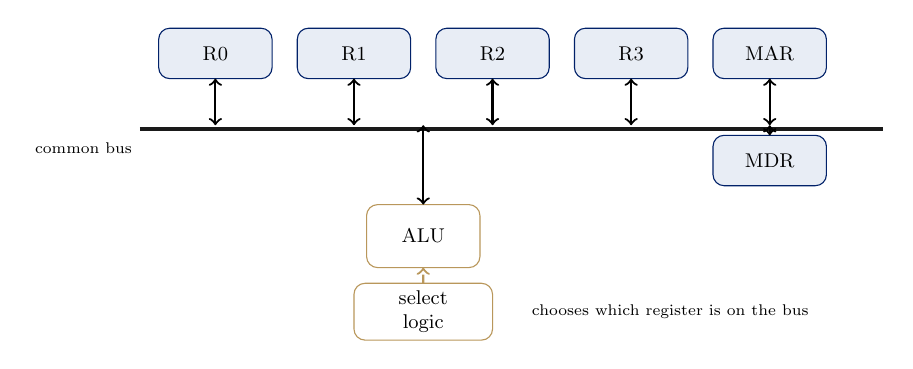
\begin{tikzpicture}[scale=0.80, transform shape,
      every node/.style={font=\small}]
    \draw[very thick, jet] (-1.2,0) -- (10.6,0);
    \node[font=\scriptsize, below left] at (-1.2,-0.1) {common bus};
    \node[draw=primary-blue, fill=light-bg, rounded corners,
          minimum width=1.8cm, minimum height=0.8cm, align=center] (R0) at (0,1.2) {R0};
    \node[draw=primary-blue, fill=light-bg, rounded corners,
          minimum width=1.8cm, minimum height=0.8cm, align=center] (R1) at (2.2,1.2) {R1};
    \node[draw=primary-blue, fill=light-bg, rounded corners,
          minimum width=1.8cm, minimum height=0.8cm, align=center] (R2) at (4.4,1.2) {R2};
    \node[draw=primary-blue, fill=light-bg, rounded corners,
          minimum width=1.8cm, minimum height=0.8cm, align=center] (R3) at (6.6,1.2) {R3};
    \foreach \x in {0, 2.2, 4.4, 6.6} { \draw[<->, thick] (\x,0.8) -- (\x,0.06); }
    \node[draw=primary-gold, fill=white, rounded corners,
          minimum width=1.8cm, minimum height=1.0cm, align=center] (ALU) at (3.3,-1.7) {ALU};
    \draw[<->, thick] (3.3,0.06) -- (3.3,-1.2);
    \node[draw=primary-blue, fill=light-bg, rounded corners,
          minimum width=1.8cm, minimum height=0.8cm, align=center] (MAR) at (8.8,1.2) {MAR};
    \node[draw=primary-blue, fill=light-bg, rounded corners,
          minimum width=1.8cm, minimum height=0.8cm, align=center] (MDR) at (8.8,-0.5) {MDR};
    \draw[<->, thick] (8.8,0.8) -- (8.8,0.06);
    \draw[<->, thick] (8.8,-0.1) -- (8.8,0.06);
    \node[draw=primary-gold, fill=white, rounded corners,
          minimum width=2.2cm, minimum height=0.8cm, align=center] (DEC) at (3.3,-2.9) {select\\logic};
    \draw[->, thick, primary-gold, dashed] (DEC.north) -- (3.3,-2.2);
    \node[font=\scriptsize, anchor=west] at (4.9,-2.9) {chooses which register is on the bus};
  \end{tikzpicture}
  \caption{The common bus system --- cf.\ Mano, Fig.~5-4, p.129. One shared path carries values among registers, ALU, and memory; the select unit (decoder) chooses which register drives the bus each cycle.}
  \label{fig:common-bus}
\end{figure}

\textbf{How to present it:} draw the single horizontal bus first, labeled \emph{common bus}, then the four registers above it one at a time, each with its vertical connection, then the ALU and the \texttt{MAR}/\texttt{MDR} memory interface on the right, then the \texttt{select logic} box below --- saving its label for last, so the class guesses what it does. The vertical ``tap'' into the ALU should be centered under the ALU's column so it reads cleanly.

\begin{teachingaside}
Students routinely ask why every register needs its own wire to the bus rather than ``just connecting R1 to R2 directly.'' The answer is exactly the bus's reason to exist: $n$ registers with all pairwise wires is $n(n-1)/2$ wires, but one bus is $n$ taps. Say the count out loud --- it is the same ``shared medium'' argument as a class room's single whiteboard.
\end{teachingaside}

Now the selection mechanism (Mano, Table~8-1, p.243): \texttt{SELA} names which register's contents go to the ALU's \emph{first} input; \texttt{SELB} names which register's contents go to the ALU's \emph{second} input; \texttt{SELD} names \emph{which} register is loaded with the result. The idea: register selection is \emph{encoded} in a few select bits and decoded into one-hot ``drive bus'' / ``load now'' signals --- that is the whole trick behind moving values between registers without hard-wiring every pair.

\begin{example}[\texttt{R1} $\gets$ \texttt{[R2]} over the common bus]
Copy the \emph{contents} of \texttt{R2} into \texttt{R1} (contents of register X are written $[X]$):
\begin{enumerate}
  \item \texttt{SELA} encodes ``\texttt{R2}'' --- R2's output enable goes high.
  \item \texttt{R2}'s contents are driven onto the common bus.
  \item \texttt{SELD} encodes ``\texttt{R1}'' --- R1's load-enable goes high.
  \item On the clock edge, \texttt{R1} captures whatever the bus holds: $R1 \gets [R2]$.
\end{enumerate}
No direct \texttt{R2}$\to$\texttt{R1} wire exists --- every transfer uses the bus plus two select signals.
\end{example}

\textbf{A question worth asking live}, after the trace: ``what would change if we wanted \texttt{R1} $\gets$ \texttt{R3} instead?'' (Nothing structural --- only the encoded values of \texttt{SELA} and \texttt{SELD} change.) This is the payoff question that shows the bus + select mechanism is generic.

\begin{teachingaside}
The single most likely point of confusion is conflating \texttt{SELA}/\texttt{SELB} (which \emph{sources} feed the ALU) with \texttt{SELD} (which register \emph{receives} the result). Drill the asymmetry: two source-select fields, one destination-select field, because an ALU operation has two operands but one result.
\end{teachingaside}

\begin{example}[A Second Instance: \texttt{R3} $\gets$ \texttt{[R0]} $+$ \texttt{[R2]}]
\begin{enumerate}
  \item \texttt{SELA} = ``\texttt{R0}'' --- R0's contents driven onto the bus into ALU input A.
  \item \texttt{SELB} = ``\texttt{R2}'' --- R2's contents driven onto the bus into ALU input B.
  \item ALU set to add; \texttt{SELD} = ``\texttt{R3}'' --- R3's load-enable goes high.
  \item On the clock edge, $R3 \gets [R0]+[R2]$.
\end{enumerate}
Identical machinery to the copy example --- the only new element is the ALU's select line between steps 2 and 3.
\end{example}

Close the section with the Socratic check: why not put \emph{everything} in registers? Registers are scarce (a few dozen at most), costly (silicon area + power for each), so they are a scratchpad for what is \emph{being} worked on; values rest in memory (big, cheap, persistent) and are loaded in only while the ALU touches them. Ask the question live and let the class produce ``scarcity'' and ``cost'' before you confirm.

\section{Stack Organization}

Pose the postfix puzzle: how would a calculator evaluate \texttt{A B +} if it could only look at the \emph{top} item of a scratch list --- no registers, no random access? The rule: read a value, \key{push} it; read an operator, \key{pop} the last two values, compute, \key{push} the result. The \emph{last} value pushed is the \emph{first} taken back out --- \key{last-in, first-out} (LIFO). That is a \key{stack}. Name the machines that use it: HP calculators, the JVM.

\begin{definitionbox}{Stack}
An ordered storage structure where all insertions and deletions happen at \emph{one end}, the \textbf{top}, addressed by a dedicated register \texttt{SP} (the \key{stack pointer}); behavior is LIFO (Mano, Sec.~8-3, p.247).
\end{definitionbox}

\textbf{PUSH:} $SP \gets [SP] - 1$, then $M[SP] \gets$ operand --- store at the new top (the stack grows \emph{downward} toward lower addresses). \textbf{POP:} operand $\gets M[SP]$, then $SP \gets [SP] + 1$ --- remove the current top.

\begin{teachingaside}
The downward growth (decrement on PUSH, increment on POP) is the \#1 intuition inversion of the whole lecture --- every student assumes a stack grows \emph{up}. State the convention loudly and give the reason: the stack shares memory with the rest of the program, and growing downward from a high base keeps it from colliding with the low-addressed program/data region.
\end{teachingaside}

\begin{example}[PUSH and POP micro-transfers]
Stack contains \texttt{[? , 5 , 7]} with top at 7. \texttt{PUSH 9} $\Rightarrow$ \texttt{[? , 5 , 7 , 9]}; \texttt{POP} $\Rightarrow$ returns 9, stack back to \texttt{[? , 5 , 7]}.
\end{example}

Then run the \texttt{A + B} stack trace (Table~\ref{tab:stack-add}) and stop at the ADD row: this instruction names \emph{no operands at all} --- both come implicitly from the top of the stack. That is the \key{zero-address} format, met properly in the next section.

\begin{table}[h]
\centering
\small
\begin{tabular}{@{}clp{4.2cm}p{4.2cm}@{}}
\toprule
\textbf{Step} & \textbf{Operation} & \textbf{Stack after (top right)} & \textbf{Effect} \\
\midrule
1 & \texttt{PUSH A} & \texttt{A} & value A stored at top \\
2 & \texttt{PUSH B} & \texttt{B A} & value B stored above A \\
3 & \texttt{ADD}    & \texttt{A+B} & pop B, pop A, push result \\
4 & \texttt{POP X}  & \emph{empty} & store top into \texttt{X} \\
\bottomrule
\end{tabular}
\caption{\texttt{A + B} on a stack machine --- the \texttt{ADD} names no operands; both come from the stack top.}
\label{tab:stack-add}
\end{table}

Now the two hardware homes (Mano, Sec.~8-3, p.248): a \key{register stack} lives inside the CPU in a set of registers --- very fast but only a handful of words (e.g.\ 64); a \key{memory stack} is a region of main memory with \texttt{SP} holding the address of the top --- as large as memory, but every PUSH/POP is a memory access. Real machines choose memory stacks because function calls nest deeply (recursion); real ISAs keep \texttt{SP} in a register and store frames in memory (P\&H, Sec.~2.8, p.100). Say the punchline: registers are the pointer, memory is the stack.

\begin{example}[A Second Instance: \texttt{A} $-$ \texttt{B} on a stack machine]
\texttt{PUSH A; PUSH B; SUB; POP X} --- the \texttt{SUB} again names no operands. Worth asking: which order does the ALU pop them in, so that $A-B$ (not $B-A$) is computed? (The \emph{second}-popped value is the minuend --- convention matters and is worth one live question.)
\end{example}

Close with the registers-vs-stack check: a stack restricts access (only the top --- no random access mid-computation), costs reordering when a buried value is needed (pop everything above it first), but shrinks instructions (operands implicit --- hence the compact zero-address format). Compilers love the compactness; hardware pays with restricted access.

\section{Instruction Formats}

Pose the question that defines the section: the CPU must be told \emph{what} to do and \emph{where} the operands are. How much ``where'' information must a machine instruction physically carry? At minimum an \key{opcode}; beyond that, \emph{addresses} --- and each address costs bits. The trade-off is fundamental: more addresses per instruction $\Rightarrow$ more work done per instruction but longer instructions; fewer addresses $\Rightarrow$ compact but more instructions, and the hardware must know where the operands are implicitly.

\begin{definitionbox}{Instruction Format}
The layout of an instruction word: an \textbf{opcode} field naming the operation, followed by zero or more \textbf{address/operand} fields naming where operands and results live (Mano, Sec.~8-4, p.255).
\end{definitionbox}

Fields are fixed-width bits; the opcode width sets an upper bound on how many distinct instructions the ISA can name. P\&H's LEGv8 shows the fixed-width idea concretely --- instructions in a handful of formats (R/I/IS/B/CB/IM), each with fixed fields (P\&H, Sec.~2.5, p.82).

\begin{figure}[h]
  \centering
  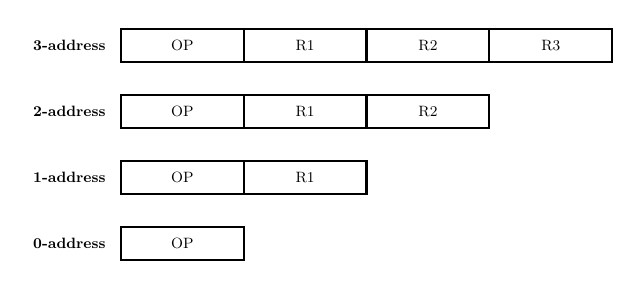
\begin{tikzpicture}[scale=0.6, transform shape,
      every node/.style={font=\small}]
    \draw[thick] (0,0) rectangle (10.4,-0.7);
    \draw[thick] (2.6,0) -- (2.6,-0.7);  \draw[thick] (5.2,0) -- (5.2,-0.7);
    \draw[thick] (7.8,0) -- (7.8,-0.7);
    \node at (1.3,-0.35) {OP}; \node at (3.9,-0.35) {R1};
    \node at (6.5,-0.35) {R2}; \node at (9.1,-0.35) {R3};
    \node[left] at (-0.2,-0.35) {\textbf{3-address}};
    \draw[thick] (0,-1.4) rectangle (7.8,-2.1);
    \draw[thick] (2.6,-1.4) -- (2.6,-2.1);  \draw[thick] (5.2,-1.4) -- (5.2,-2.1);
    \node at (1.3,-1.75) {OP}; \node at (3.9,-1.75) {R1}; \node at (6.5,-1.75) {R2};
    \node[left] at (-0.2,-1.75) {\textbf{2-address}};
    \draw[thick] (0,-2.8) rectangle (5.2,-3.5);
    \draw[thick] (2.6,-2.8) -- (2.6,-3.5);
    \node at (1.3,-3.15) {OP}; \node at (3.9,-3.15) {R1};
    \node[left] at (-0.2,-3.15) {\textbf{1-address}};
    \draw[thick] (0,-4.2) rectangle (2.6,-4.9);
    \node at (1.3,-4.55) {OP};
    \node[left] at (-0.2,-4.55) {\textbf{0-address}};
  \end{tikzpicture}
  \caption{The four instruction-format families --- cf.\ Mano, Sec.~8-4, p.255: as the operand count falls, instructions get shorter but the machine must find operands implicitly.}
  \label{fig:format-families}
\end{figure}

\textbf{How to present it:} draw the four rows \emph{top to bottom} and read them as a compression story. Draw the 3-address row fully (OP + three fields), then ask the class to predict what the 2-address row drops, and so on down to 0-address (OP only). The visual of words shrinking while ``implicit operand'' grows is the entire section in one figure.

State each family's rule clearly:
\begin{itemize}
  \item \textbf{3-address:} \texttt{ADD R1, R2, R3} $\Rightarrow$ $R1 \gets [R2]+[R3]$ --- all explicit; the most flexible, longest form; register ISAs (RISC).
  \item \textbf{2-address:} \texttt{ADD R1, R2} $\Rightarrow$ $R1 \gets [R1]+[R2]$ --- the first field doubles as one operand \emph{and} the result; \key{destructive} (old \texttt{R1} lost); older CISC.
  \item \textbf{1-address:} \texttt{ADD A} $\Rightarrow$ $AC \gets [AC]+[A]$ --- one operand is always the accumulator \texttt{AC}, named by no field; simple CPUs.
  \item \textbf{0-address:} \texttt{ADD} $\Rightarrow$ pop two, push sum --- \emph{only} the opcode; every operand implicit from the stack top; stack machines, JVM.
\end{itemize}

\begin{teachingaside}
The word \key{destructive} (2-address) needs an explicit example, not just a definition --- students accept ``\texttt{ADD R1,R2} loses \texttt{R1}'s old value'' only when they see it force an extra \texttt{MOV} into the program (below). Tie it forward: this is \emph{why} the 2-address program is longer than the 3-address one.
\end{teachingaside}

Now the running thread, compiled in every format. Write each tally on the board and let the class count with you.

\begin{example}[3-address: \texttt{X = (A+B)$\times$(C+D)}]
\texttt{ADD R1, A, B} $\Rightarrow$ $R1 \gets A+B$; \quad \texttt{ADD R2, C, D} $\Rightarrow$ $R2 \gets C+D$; \quad \texttt{MUL X, R1, R2} $\Rightarrow$ $X \gets R1 \times R2$.\\
\textbf{3 instructions}, each carrying three addresses --- wide words, short program, no extra data movement.
\end{example}

\begin{example}[2-address: the same expression]
\texttt{MOV R1, A; ADD R1, B; MOV R2, C; ADD R2, D; MUL X, R1} (R2 is the implicit second operand of \texttt{MUL}).\\
\textbf{5 instructions} vs.\ 3 --- the 2-address format is cheaper per instruction but needs extra copy instructions because \texttt{ADD} is destructive.
\end{example}

\begin{example}[1-address: the same expression]
\texttt{LOAD A; ADD B; STORE T; LOAD C; ADD D; MUL T; STORE X} --- with a temporary \texttt{T} in memory, because the accumulator cannot hold two partial results at once.\\
\textbf{7 instructions.}
\end{example}

\begin{example}[0-address: the same expression]
\texttt{PUSH A; PUSH B; ADD; PUSH C; PUSH D; ADD; MUL; POP X} --- shortest instructions, but the most of them.\\
\textbf{8 instructions.}
\end{example}

\textbf{A question worth asking live}, after the 3-address tally: ``what is the one instruction the 3-address program never needs that the 2-address program does?'' (The \texttt{MOV}/\texttt{LOAD} copies --- 3-address has no destructive overwrite to repair.) Then put all four counts on the board at once (Table~\ref{tab:format-summary}).

\begin{table}[h]
\centering
\small
\renewcommand{\arraystretch}{1.15}
\begin{tabular}{@{}p{1.8cm}p{2.4cm}p{4.0cm}p{2.2cm}p{2.6cm}@{}}
\toprule
\textbf{Format} & \textbf{Example} & \textbf{Program size for }$X=(A{+}B)\times(C{+}D)$ & \textbf{Operand access} & \textbf{Typical use} \\
\midrule
3-address & \texttt{ADD R1,R2,R3} & 3 instr., wide words & all explicit & register ISAs (RISC) \\
2-address & \texttt{ADD R1,R2}    & 5 instr. + copies     & one destroyed      & older CISC \\
1-address & \texttt{ADD A}        & 7 instr., needs temps & accumulator        & simple CPUs \\
0-address & \texttt{ADD}          & 8 instr., compact    & stack top          & stack machines, JVM \\
\bottomrule
\end{tabular}
\caption{The four formats side by side --- cf.\ Mano, Sec.~8-4, p.255.}
\label{tab:format-summary}
\end{table}

\begin{teachingaside}
Resist the urge to call any format ``best.'' The class will want a winner. The correct takeaway is the monotone trade-off: fewer addresses $\Rightarrow$ more instructions but compact words; more addresses $\Rightarrow$ fewer instructions but wide words. RISC uses 3-address; the JVM uses 0-address; both are correct for their design goals.
\end{teachingaside}

\section{Instruction Cycle}

Set up the section with the Socratic question: \texttt{ADD R1, A} sits in memory; for it to take effect the CPU must bring it in, understand it, collect \texttt{[R1]} and \texttt{[A]}, add, and store back. What fixed sequence of basic steps does the machine repeat for \emph{every} instruction? The answer is the \key{instruction cycle} --- a skeleton the control unit runs once per instruction, identical for every instruction except that the \key{execute} phase varies by opcode.

\begin{definitionbox}{Instruction Cycle}
The fixed sequence of phases --- fetch, decode, execute --- the control unit repeats once per instruction; only the execute phase varies with the opcode.
\end{definitionbox}

\begin{figure}[h]
  \centering
  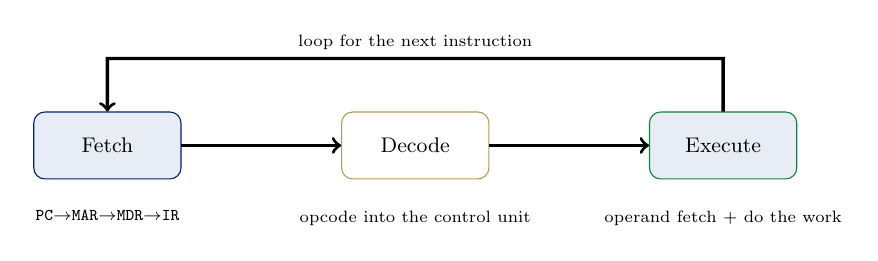
\begin{tikzpicture}[scale=0.85, transform shape,
      every node/.style={font=\small}]
    \node[draw=primary-blue, fill=light-bg, rounded corners,
          minimum width=2.2cm, minimum height=1.0cm, align=center] (F) at (0,0) {Fetch};
    \node[draw=primary-gold, fill=white, rounded corners,
          minimum width=2.2cm, minimum height=1.0cm, align=center] (D) at (4.6,0) {Decode};
    \node[draw=positive, fill=light-bg, rounded corners,
          minimum width=2.2cm, minimum height=1.0cm, align=center] (E) at (9.2,0) {Execute};
    \draw[->, very thick] (F.east) -- (D.west);
    \draw[->, very thick] (D.east) -- (E.west);
    \draw[->, very thick] (E.north) -- (9.2,1.3) -- (0,1.3) -- (F.north);
    \node[font=\scriptsize, above] at (4.6,1.3) {loop for the next instruction};
    \node[font=\scriptsize, below] at (0,-0.85) {\texttt{PC}$\to$\texttt{MAR}$\to$\texttt{MDR}$\to$\texttt{IR}};
    \node[font=\scriptsize, below] at (4.6,-0.85) {opcode into the control unit};
    \node[font=\scriptsize, below] at (9.2,-0.85) {operand fetch + do the work};
  \end{tikzpicture}
  \caption{The instruction cycle --- fetch, decode, execute --- as a loop (Hamacher, \textit{Computer Organization}, Ch.~7; standard treatment).}
  \label{fig:instruction-cycle}
\end{figure}

\textbf{How to present it:} draw the three boxes left to right first, then the return arrow across the top last --- and narrate the top arrow as the thing that makes it a \emph{cycle}: ``after execute, we go back and fetch the next instruction.'' The three sub-captions under the boxes (\texttt{PC}$\to$\texttt{MAR}$\to$\texttt{MDR}$\to$\texttt{IR}; opcode into control unit; operand fetch + do the work) should each be revealed as you explain that phase.

\begin{teachingaside}
Students often think decode and execute are the ``interesting'' phases and fetch is trivial bookkeeping. The teaching move is the reverse emphasis: fetch is the \emph{identical} prologue every instruction runs, and it is where \texttt{PC}, \texttt{MAR}, \texttt{MDR}, \texttt{IR} all earn their keep at once. Spend the time on fetch's five transfers; execute's variety is then a natural surprise rather than a laundry list.
\end{teachingaside}

Spell out fetch's five transfers (the sub-caption under the Fetch box, expanded): \texttt{MAR} $\gets$ \texttt{[PC]}; initiate a memory read at \texttt{MAR}; \texttt{MDR} $\gets$ \emph{memory data}; \texttt{IR} $\gets$ \texttt{[MDR]}; \texttt{PC} $\gets$ \texttt{[PC]} $+1$. Each register exists for \emph{one} reason: \texttt{PC} holds the next address, \texttt{MAR} pins it during the access, \texttt{MDR} buffers the incoming word, \texttt{IR} holds the current instruction while it is decoded.

\textbf{A question worth asking live}, after the five transfers: ``why does the instruction go \texttt{PC} $\to$ \texttt{MAR} $\to$ \texttt{MDR} $\to$ \texttt{IR} instead of straight \texttt{PC} $\to$ \texttt{IR}?'' (Because \texttt{PC} and \texttt{IR} are not connected by a direct path in a bus machine --- the memory interface needs the address pinned in \texttt{MAR} for the whole access and the word buffered in \texttt{MDR} before it is stable enough to load into \texttt{IR}.)

Then decode and execute. Decode: the opcode bits of \texttt{IR} tell the control unit \emph{which} operation this is --- it then selects the right sequence of control signals (exactly what Weeks~6--7 build). Execute: the operand-dependent part --- if a memory operand is needed, its address is resolved (addressing modes, Week 5) and the operand fetched into a register; the ALU performs the operation; the result is written to the destination named in the instruction. The \emph{number} of execute steps varies by instruction --- fetch is fixed, execute is not.

\begin{example}[One full cycle for \texttt{ADD R1, A}]
\begin{center}
\small
\begin{tabular}{@{}cp{3.4cm}p{3.6cm}p{3.4cm}@{}}
\toprule
\textbf{Phase} & \textbf{Register activity} & \textbf{Memory / ALU} & \textbf{State} \\
\midrule
Fetch &
  \texttt{MAR}$\gets$\texttt{[PC]}; \texttt{MDR}$\gets$instr.; \texttt{IR}$\gets$\texttt{[MDR]}; \texttt{PC}$\gets$\texttt{[PC]}$+1$ &
  read instruction word &
  instruction in \texttt{IR} \\
Decode &
  \texttt{IR} opcode $\to$ control unit &
  --- &
  operation identified \\
Execute &
  operand \texttt{[A]} fetched; \texttt{AC}$\gets$\texttt{[AC]}+\texttt{[A]} &
  read operand; ALU adds &
  result in \texttt{AC} \\
\bottomrule
\end{tabular}
\end{center}
The same three phases run for every instruction --- only the execute row changes.
\end{example}

\begin{example}[A Second Instance: \texttt{STORE X} on the same machine]
Fetch (identical five transfers, \texttt{PC} incremented); decode (opcode = \texttt{STORE}); execute (the operand \texttt{[X]}'s \emph{address} is resolved, the value to store is already in \texttt{AC}, and the memory write is issued --- note the execute row here writes \emph{out} rather than reading in, so its register activity and memory column differ completely from \texttt{ADD}). Use this contrast to make the point that only the execute row varies.
\end{example}

Now the four types of operands (Hamacher, Ch.~7; standard treatment): \key{addresses} (a location in memory --- used by \texttt{LOAD}, \texttt{STORE}, \texttt{BRANCH}); \key{numbers} (integer or floating-point values the ALU computes on); \key{characters} (text --- usually ASCII/Unicode codes in a byte or halfword); \key{logical data} (bit patterns --- each bit its own value; \texttt{AND}, \texttt{OR}, \texttt{XOR}, shifts work bitwise). Why this matters: the \emph{type} determines how the ALU wires the bits --- a branch needs the address, an integer add needs the value, a shift needs the bit mask --- and the opcode says which interpretation applies (P\&H makes the same operand taxonomy in Sec.~2.3, p.67).

\begin{teachingaside}
The four operand types are the section's ``so what.'' Without them, the cycle looks like pointless plumbing; with them, the fetch--decode--execute skeleton becomes \emph{the} engine that interprets whichever kind of data the opcode names. Connect each type to the ALU operation it feeds (branch $\to$ address, add $\to$ value, shift $\to$ mask) as you list it.
\end{teachingaside}

Close the section by tying the week together on the board: for \texttt{ADD R1, A} on an accumulator machine, \texttt{PC} points at the next instruction; \texttt{IR} holds the current one after fetch; the first operand is \texttt{AC} (the implicit operand of the 1-address format); the second is memory location \texttt{A}, fetched during execute. Every piece of that answer came from the register organization, the formats, and the cycle --- one connected machine.

\section{Synthesis and Summary}

Storage spaces and formats are two sides of one choice: \key{registers} (fast, explicit, random access) buy the wide 3-address format; \key{stack} (compact, restricted, implicit) buys the 0-address format; the instruction cycle is the glue that steps whichever format the ISA chose through the same fetch/decode/execute skeleton. The running thread closes: $X = (A+B)\times(C+D)$ ran in 3, 5, 7, or 8 instructions depending on the format, and each of those instructions then lives through one full fetch--decode--execute cycle.

Set up next week's hook explicitly: we wrote ``\texttt{ADD R1, A}'' and said ``operand \texttt{[A]} is fetched'' --- but never how the field \texttt{A} turns into the actual location of the operand. That is \key{addressing modes}, Week 5, together with the datapath (buses) that actually moves the values.

\textbf{Summary --- quick reference:} \emph{Register organization:} registers are the one-cycle scratchpad; transfers happen over a common bus selected by \texttt{SELA}/\texttt{SELB}/\texttt{SELD}. \emph{Stack organization:} \texttt{SP} addresses a LIFO top; PUSH/POP with $\pm 1$ on \texttt{SP}; register stacks fast, memory stacks large. \emph{Instruction formats:} 3-, 2-, 1-, 0-address --- the address count trades instruction width against program size (3 vs.\ 5 vs.\ 7 vs.\ 8 instructions for one expression). \emph{Instruction cycle:} fetch (\texttt{PC}$\to$\texttt{MAR}$\to$\texttt{MDR}$\to$\texttt{IR}, \texttt{PC}${+}1$), decode, execute. \emph{Operand types:} addresses, numbers, characters, logical data --- the opcode picks the interpretation.

\end{document}
